\documentclass[APA,LATO1COL,doublespace]{WileyNJD-v2}
%DIF LATEXDIFF DIFFERENCE FILE
%DIF DEL paper-SMapp-1st/SMapp.tex   Fri Feb  7 12:50:24 2020
%DIF ADD paper-SMapp-2nd/SMapp.tex   Fri Feb  7 12:48:48 2020
\usepackage{moreverb}

% Giuliano
%DIF 5a5
\usepackage{lineno} %DIF > 
%DIF -------
\usepackage{graphicx}
%DIF 6c7-8
%DIF < \graphicspath{ {Figures/} }
%DIF -------
\graphicspath{ {EPS/} } %DIF > 
%\graphicspath{ {Figures/} } %DIF > 
%DIF -------
\usepackage{enumitem} % to have (i) bulletts
%
% ==== REVIEW ONLY ====
% http://texdoc.net/texmf-dist/doc/latex/endfloat/endfloat.pdf
% tables and figures at the end of document
\usepackage[notablist,figlist,tablesfirst]{endfloat}
% =====================
%
% == COMMENT AFTER EDITOR APPROVAL ABOUT LENGTH OF PAPER ==
%\usepackage{draftwatermark}
%\SetWatermarkText{Ed. approval}
%\SetWatermarkScale{1.0} % size of the watermark
% =========================================================
%
% ==== ADD ORCID REFERENCE ====
% git repo :: https://github.com/diogo-fernan/academicons
%
%    **ATTEMPT #1**
% See link https://tex.stackexchange.com/questions/275578/is-there-a-standard-way-to-include-orcid-in-tex-pdf
%\usepackage{./academicons}
%\newcommand{\myOrcid}[1]{\href{https://orcid.org/#1}{\textcolor[HTML]{A6CE39}{\aiOrcid}}}
%\definecolor{orcidlogocol}{HTML}{A6CE39}
%
%    **ATTEMPT #2**
% https://tex.stackexchange.com/questions/445563/ieeetran-how-to-include-orcid-in-tex-pdf-with-pdflatex
\usepackage{scalerel}
\usepackage{tikz}
\usetikzlibrary{svg.path}
\definecolor{orcidlogocol}{HTML}{A6CE39}
\tikzset{
  orcidlogo/.pic={
    \fill[orcidlogocol] svg{M256,128c0,70.7-57.3,128-128,128C57.3,256,0,198.7,0,128C0,57.3,57.3,0,128,0C198.7,0,256,57.3,256,128z};
    \fill[white] svg{M86.3,186.2H70.9V79.1h15.4v48.4V186.2z}
                 svg{M108.9,79.1h41.6c39.6,0,57,28.3,57,53.6c0,27.5-21.5,53.6-56.8,53.6h-41.8V79.1z M124.3,172.4h24.5c34.9,0,42.9-26.5,42.9-39.7c0-21.5-13.7-39.7-43.7-39.7h-23.7V172.4z}
                 svg{M88.7,56.8c0,5.5-4.5,10.1-10.1,10.1c-5.6,0-10.1-4.6-10.1-10.1c0-5.6,4.5-10.1,10.1-10.1C84.2,46.7,88.7,51.3,88.7,56.8z};
  }
}
\newcommand\orcidicon[1]{\href{https://orcid.org/#1}{\mbox{\scalerel*{

\begin{tikzpicture}[yscale=-1,transform shape]
\pic{orcidlogo};
\end{tikzpicture}
}{|}}}}
\usepackage{hyperref} %<--- Load after everything else
% =============================
%
%\usepackage{array}
%\usepackage{cleveref}
%\usepackage{siunitx}

\newcommand\BibTeX{{\rmfamily B\kern-.05em \textsc{i\kern-.025em b}\kern-.08em
T\kern-.1667em\lower.7ex\hbox{E}\kern-.125emX}}

\articletype{Research Article}%

\received{<day> <Month>, <year>}
\revised{<day> <Month>, <year>}
\accepted{<day> <Month>, <year>}

%\raggedbottom
 %DIF > 
\linenumbers %DIF > 
%DIF PREAMBLE EXTENSION ADDED BY LATEXDIFF
%DIF UNDERLINE PREAMBLE %DIF PREAMBLE
%\RequirePackage[normalem]{ulem} %DIF PREAMBLE
\PassOptionsToPackage{normalem}{ulem}
\RequirePackage{color}\definecolor{RED}{rgb}{1,0,0}\definecolor{BLUE}{rgb}{0,0,1} %DIF PREAMBLE
\providecommand{\DIFaddtex}[1]{{\protect\color{blue}\uwave{#1}}} %DIF PREAMBLE
\providecommand{\DIFdeltex}[1]{{\protect\color{red}\sout{#1}}}                      %DIF PREAMBLE
%DIF SAFE PREAMBLE %DIF PREAMBLE
\providecommand{\DIFaddbegin}{} %DIF PREAMBLE
\providecommand{\DIFaddend}{} %DIF PREAMBLE
\providecommand{\DIFdelbegin}{} %DIF PREAMBLE
\providecommand{\DIFdelend}{} %DIF PREAMBLE
%DIF FLOATSAFE PREAMBLE %DIF PREAMBLE
\providecommand{\DIFaddFL}[1]{\DIFadd{#1}} %DIF PREAMBLE
\providecommand{\DIFdelFL}[1]{\DIFdel{#1}} %DIF PREAMBLE
\providecommand{\DIFaddbeginFL}{} %DIF PREAMBLE
\providecommand{\DIFaddendFL}{} %DIF PREAMBLE
\providecommand{\DIFdelbeginFL}{} %DIF PREAMBLE
\providecommand{\DIFdelendFL}{} %DIF PREAMBLE
%DIF END PREAMBLE EXTENSION ADDED BY LATEXDIFF
%DIF PREAMBLE EXTENSION ADDED BY LATEXDIFF
%DIF HYPERREF PREAMBLE %DIF PREAMBLE
\providecommand{\DIFadd}[1]{\texorpdfstring{\DIFaddtex{#1}}{#1}} %DIF PREAMBLE
\providecommand{\DIFdel}[1]{\texorpdfstring{\DIFdeltex{#1}}{}} %DIF PREAMBLE
%DIF END PREAMBLE EXTENSION ADDED BY LATEXDIFF

\begin{document}

\title{Soil Monitor: an internet platform to challenge soil sealing in Italy}

\author[1,2]{Giuliano Langella*}
\author[2,3]{Angelo Basile}
\author[4]{Simone Giannecchini}
\author[5,6]{Francesco Domenico Moccia}
\author[1]{Florindo Antonio Mileti}
\author[7]{Michele Munaf\'o}
\author[8]{Francesco Pinto}
\author[1,2]{Fabio Terribile}
\authormark{LANGELLA \textsc{et al}}

%\address[1]{\orgdiv{Org Division}, \orgname{Org name}, \orgaddress{\state{State name}, \country{Country name}}}
\address[1]{\orgdiv{Department of Agriculture}, \orgname{Universit\'a di Napoli Federico II}, \orgaddress{via Universit\'a 100, Portici 80055, \state{Napoli}, \country{Italy}}}

\address[2]{\orgdiv{Interdepartmental Centre on Earth Critical Zone (CRISP)}, \orgname{Universit\'a di Napoli Federico II}, \orgaddress{via Universit\'a 100, Portici 80055, \state{Napoli}, \country{Italy}}}

\address[3]{\orgdiv{ISAFom Institute}, \orgname{National Research Council}, \orgaddress{via Patacca 85, Ercolano 80056, \state{Napoli}, \country{Italy}}}

\address[4]{\orgname{GeoSolutions S.A.S.}, \orgaddress{via di Montramito 3/A, Massarosa 55054, \state{Lucca}, \country{Italy}}}

\address[5]{\orgdiv{Department of Architecture}, \orgname{Universit\'a di Napoli Federico II}, \orgaddress{via Toledo 402, Napoli 80134, \state{Napoli}, \country{Italy}}}

\address[6]{\orgname{Istituto Nazionale di Urbanistica (INU)}, \orgaddress{Via Castro dei Volsci 14, Roma 00179 \state{Roma}, \country{Italy}}}

\address[7]{\orgname{Istituto Superiore per la Protezione e la Ricerca Ambientale (ISPRA)}, \orgaddress{Via Brancati 48, Roma 00144 \state{Roma}, \country{Italy}}}

\address[8]{\orgname{EMM S.R.L.}, \orgaddress{via Vicinale Santa Maria del Pianto, Napoli 80143 \state{Napoli}, \country{Italy}}}


\corres{*Giuliano Langella, Department of Agriculture, Universit\'a di Napoli Federico II. \email{glangella@unina.it}}

\presentaddress{via Universit\'a 100, 80055 Portici, Italy}

\DIFaddbegin \abstract[ Abstract ]{
This work propose a new type of web-based geospatial decision support system --- called Soil Monitor --- which provides a multidisciplinary operational tool useful for a multi-stakeholder community to challenge soil sealing.
Different technological and technical features of Soil Monitor are presented and discussed with particular reference to the combination of WebGIS with on-the-fly geospatial processing based on GPU computing, specifically designed to allow real-time requests.
In addition, we present three quantitative analysis about soil sealing at three different scales.
The study at national level illustrated that the type of land use strongly affected soil sealing dynamics.
Indeed, the class \textit{complex cultivation pattern} resulted the most fragile land use while \textit{forests} resulted the most resilient one.
The study at province level illustrated the key importance of having on-the-fly the map of rural fragmentation for any Italian province.
This map --- quantifying the integrity of the rural territory --- enables to better locate both new green corridors or new urban development lowering the impact over the rural environment.
The study at municipality level (Napoli) demonstrated the importance of quantifying a pool of spatial planning indicators and illustrated that (i) the largest urban dispersion occurs in hilly touristic municipalities close to the sea, (ii) the increase in soil sealing in rural sites is not justified by population growth.
As a result, Soil Monitor is deemed useful both to support decision making at different spatial scales and to raise awareness in people, professionals, and experts of other fields.
}
\DIFaddend 

\keywords{soil sealing, geospatial decision support system, CUDA, GPU computing, urban planning}
%Class file; \LaTeXe; \emph{Wiley NJD}}

\jnlcitation{
\cname{%
    \author{Langella G.}, 
    \author{A. Basile}, 
    \author{S. Giannecchini}, 
    \author{F.D. Moccia}, 
    \author{F.A. Mileti},
    \author{M. Munaf\'o},
    \author{F. Pinto} and
    \author{F. Terribile}
}
(\cyear{<year>}), 
\ctitle{Soil Monitor: an internet platform to challenge soil sealing in Italy},
\cjournal{Land Degradation \& Development}, \cvol{<year>;<number>:<page>--<page>}.}

\maketitle

%DIF < \footnotetext{\textbf{Abbreviations:} ANA, anti-nuclear antibodies; APC, antigen-presenting cells; IRF, interferon regulatory factor}
\DIFaddbegin \footnotetext{\textbf{\DIFadd{Abbreviations:}}
%DIF > abbreviation, meaning; 
\DIFadd{CLC, Corine Land Cover;
CUDA, Compute Unified Device Architecture;
ED, Edge Density;
GCI, Geospatial Cyber-Infrastructure;
GPU, Graphical Processing Unit;
ISPRA, Italian Institute for Environmental Protection and Research;
LCPI, Largest Class Patch Index;
LULC, Land Use and Land Cover;
NHRSC, National High-Resolution Soil Consumption;
RMPS, Residual Mean Patch Surface;
RoI, Region of Interest;
SNPA, National System for the Protection of the Environment;
WFS, Web Feature Service;
WMS, Web Map Service;
WPS, Web Processing Service
}}
\DIFaddend 

\section{Introduction}\label{sec1}
Soil sealing \DIFdelbegin \DIFdel{is one of the most serious land degradation process, which }\DIFdelend refers to covering the ground by an impermeable material \DIFaddbegin \DIFadd{and is both the most serious land degradation process in Europe and one of the most important form of land degradation worldwide \mbox{%DIFAUXCMD
\citep{FAO15}}%DIFAUXCMD
}\DIFaddend .
It is regarded as \DIFdelbegin \DIFdel{the greatest }\DIFdelend \DIFaddbegin \DIFadd{one of the most serious }\DIFaddend threat to soil functions since it strongly disturbs or removes essential ecosystem services \DIFdelbegin \DIFdel{such as food production, water absorption, rainwater infiltration, and groundwater recharge, filtering and buffering capacity of the soil, biodiversity, etc.\mbox{%DIFAUXCMD
\citep{FAO15}}%DIFAUXCMD
. Accordingly, several services of such kind are irreplaceable, such as those provided and supported by healthy soils and diverse vegetation \mbox{%DIFAUXCMD
\citep{Dunbar13}}%DIFAUXCMD
.
According to }\DIFdelend \DIFaddbegin \DIFadd{(e.g. \mbox{%DIFAUXCMD
\citealp{Calzolari16,Dunbar13}}%DIFAUXCMD
).
Moreover, }\DIFaddend the European Environmental Agency \citep{EEA2011} \DIFdelbegin \DIFdel{, }\DIFdelend \DIFaddbegin \DIFadd{highlights that }\DIFaddend land take (land converted into artificial surfaces) by cities has increased by about 80\% in the past 60 years \DIFdelbegin \DIFdel{(}\DIFdelend whereas population has grown by only 33\%\DIFdelbegin \DIFdel{); thus, soil sealing and land take are the most important issues reducing irreplaceable ecosystem services}\DIFdelend .

Several European policy documents have been produced to tackle the loss of ecosystem services as well as the restoration and maintenance thereof, such as the Habitats (92/43/EEC) and Birds (2009/147/EC) Directives, the Common Agriculture Policy (CAP), and the EU Biodiversity Strategy to 2020 (specifically, Target 2).
In addition to the general regulatory frameworks, important policy measures specifically dealing with ecosystem services provided by soil functions include the Thematic Strategy for Soil Protection \citep{EC2006} and implementation of the Strategy \citep{EC2012}; the Roadmap to a Resource Efficient Europe \citep{EC2011a} targeted to limit the yearly land take at the EU level by 2020 and aiming to achieve the zero net land take by 2050 in line with the \DIFdelbegin \DIFdel{RIO }\DIFdelend \DIFaddbegin \DIFadd{Rio }\DIFaddend conference in 2012; the delivery of guidelines of good practices to mitigate soil sealing \citep{SWD12}; the delivery of the United Nations agenda \citep{UN15} for sustainable development goals, specifically Goal 11 ''\textit{Make cities and human settlements inclusive, safe, resilient, and sustainable}'' \citep{Keesstra16}.
Despite the large list of regulatory frameworks, there are no signs of change at present, and soil sealing continues to increase annually \citep{FAO15} at global (e.g. Secretariat of the Convention on Biological Diversity, 2012; UN, 2014), European (e.g. \citealp{SWD12}), and national scales \citep[e.g.][Copernicus Land Monitoring Service\footnote{ http://land.copernicus.eu}]{ISPRA16,ISPRA18}.
Moreover, the causes for soil sealing are very diverse and possible actions strongly depend on where they should be taken.

In the last decade, research on soil sealing has attempted to contribute to the understanding of this challenging soil degradation process. Major effort has been undertaken for the development of suitable monitoring methodologies \citep{ISPRA18,Alvarado18} and the evaluation of the impacts over the loss of soil ecosystem services \citep{Calzolari16}. Differently, limited effort has gone into \DIFaddbegin \DIFadd{the research aims of }\DIFaddend developing operational spatial decision support tools addressing soil sealing.
This situation is unfortunate considering that there is a growing body of applications illustrating the utility of the geospatial decision support system \DIFdelbegin \DIFdel{(SDSS) }\DIFdelend and visualization tools for spatial and urban planning  \citep[e.g.][]{Bishop98,Geertman12,Carsjens07,Malczewski04,Malczewski06,Meyer08}.
In most cases, these \DIFdelbegin \DIFdel{SDSS }\DIFdelend \DIFaddbegin \DIFadd{decision support systems }\DIFaddend have been conceived and developed to address small geographical areas, such as the \DIFdelbegin \DIFdel{SDSS proposed by \mbox{%DIFAUXCMD
\citep{Piero17} }%DIFAUXCMD
}\DIFdelend \DIFaddbegin \DIFadd{one proposed by \mbox{%DIFAUXCMD
\cite{Piero17} }%DIFAUXCMD
}\DIFaddend for 13 municipalities in South Italy, or for solving few, if not one, specific problems \citep[e.g.][]{Fedra98,Meyer08,Torresan16}. %(e.g. Fedra \& Feoli, 1998; Meyer \& Grabaum, 2008; Torresan et al., 2016).

Moreover, few contributions have clearly identified that urban planning \DIFdelbegin \DIFdel{DSS }\DIFdelend \DIFaddbegin \DIFadd{decision support systems }\DIFaddend must include predictive scenario analysis \citep{Choi16,Xiang03,Volk10} and \DIFdelbegin \DIFdel{the }\DIFdelend \textit{what-if} modelling. 
\DIFdelbegin \DIFdel{In fact}\DIFdelend \DIFaddbegin \DIFadd{Indeed}\DIFaddend , this is very much required in planning procedures in order to design and evaluate the potential impact of alternative urban/rural spatial plans \citep{Hawkins02,Harms95,Choi16,vonHaaren06}. 
Furthermore, scenario analysis is crucial in Strategic Environmental Assessment (e.g. SEA and EIA EU Directives). Currently, this fundamental planning procedure is dominated by qualitative assessment methods while there is a great demand for objective and quantitative methods \citep{Choi16} to provide more accurate and quantitative predictions of the impact of a plan or project \citep{Carver03,Vanderhaegen05}.

A decision support system addressing soil sealing should rely on well-established models, algorithms, and indicators. The use of indicators to monitor and assess soil sealing is already well known \citep{King16}, and there has been a proliferation of indicators, metrics, reports, community indicators, state of the art reports, \DIFdelbegin \DIFdel{and }\DIFdelend assessment reports, etc. \citep{Maclaren96,Tanguay10}.
In addition, specific spatial resolution requirements of indicators have been greatly emphasised \citep{Jaeger08}.
Furthermore, a large set of soil sealing indicators is typically tuned to the specific geographic, environmental, and socio-economic setting under investigation.
For instance, \citet{Munafo13}, analysed the Italian territory and identified soil sealing trends in relation to the distance from the coastline or the elevation belt, to the land cover classes or the distance from neighbour urban patches.
Accordingly, references to soil sealing indicators and best practices regarding producing them in different EU countries have been reported in \citep{EC2011b} in which, for instance, the monitoring of built areas, the total amount of green areas within city boundaries, and the unpaved land areas can be found.
\DIFaddbegin \DIFadd{Definitely, despite a large body of researches dealing with this complex issue has been already produced, some steps forward must been done in order to handle law and regulation requirements for tackling soil sealing.
}\DIFaddend 

\DIFdelbegin \DIFdel{Consequently, it is }\DIFdelend %DIF >  AIMS PARAGRAPH: topic sentence (gap) -> supporting sentences (needs) -> concluding sentence (our work)
\DIFaddbegin \DIFadd{Therefore, authors stress on the current
%DIF > there exist a gap between land degradation and soil sealing issues and tools coming from research that can help stakeholders tackle these issues.
strong gap in developing and providing integrated operational tools 
dealing with soil sealing 
to support quantitative analysis, awareness building and decision making by stakeholders.
This gap is amplified by a complete lack of tools 
%DIF > dealing with soil sealing 
capable to analyze large areas, and the situation is even more difficult, considering that these tools --- to be properly operated by planners --- should also enable scenario analysis (the so called }\textit{\DIFadd{what-if}} \DIFadd{modelling).
In more detail, it is thoroughly }\DIFaddend evident that 
(i) action is required since ``future generations will not see a healthy soil coming back within their lifetime once it has been destroyed\dots'' \citep{SWD12}; 
(ii) soil sealing mitigation must embody urban and landscape planning tools \citep{Artmann14}, enabling the link of opposite socio-economic driving forces, such as urban regeneration versus environmental protection; 
(iii) inter- and trans-disciplinary studies integrating soils in the environment are required to challenge soil sealing;
(iv) a cross-topic awareness should be raised regarding soil sealing in the policy, research, and public sectors\DIFdelbegin \DIFdel{; 
and (v) there is a strong gap in building/providing integrated operational tools to support decision making over soil sealing for large areas, and the situation is even more difficult, considering that these tools --- to be properly operated by planners --- should also enable scenario analysis (}\textit{\DIFdel{what-if}} %DIFAUXCMD
\DIFdel{modelling).
}%DIFDELCMD < 

%DIFDELCMD < %%%
\DIFdel{The }\DIFdelend \DIFaddbegin \DIFadd{.
A viable solution to fill this gap fits with the }\DIFaddend general aim of \DIFdelbegin \DIFdel{this paper is to demonstrate that }\DIFdelend \DIFaddbegin \DIFadd{our work, which deals with the development of
%DIF > This paper presents
%DIF > (\toberevised{demonstrate}\reviewer{[avoid of "demonstration" and add a "clear research purpose"]} that)
}\DIFaddend a new type of geospatial \DIFdelbegin \DIFdel{DSS }\DIFdelend \DIFaddbegin \DIFadd{decision support system }\DIFaddend --- a web-based \DIFdelbegin \DIFdel{DSS}\DIFdelend \DIFaddbegin \DIFadd{decision support system}\DIFaddend , namely Soil Monitor \DIFdelbegin \DIFdel{application (SMapp) }\DIFdelend --- developed on top of Geospatial Cyber-Infrastructures (GCI) \DIFdelbegin \DIFdel{, can provide }\DIFdelend \DIFaddbegin \DIFadd{and providing }\DIFaddend a multidisciplinary operational tool useful for a multi-stakeholder community to challenge soil sealing at \DIFdelbegin \DIFdel{the entire Italian country scale. 
This system is designed to address the accountancy of soil sealing through different indicators providing operational support to urban planners, decision makers and multi stakeholders involved in landscape planning and interested in evaluating the impact of soil sealing.
This specific contribution required a different approach, the result of which is the Soil Monitor web application. 
A set of indicators can be calculated in real-time using either Italian administrative levels (NUTS2, NUTS3, and LAU2) or user-drawn Regions of Interest (RoI).Moreover, Soil Monitor uses high resolution layers produced every year by ISPRA (Italian Institute for Environmental Protection and Research) since 2015 for drawing up the yearly soil sealing report in Italy.Thus, owing to the high-performance computing embedded in its cyber infrastructure, Soil Monitor enables real-time geospatial processing while preserving a high spatial detail of the analysis over large areas (till LAU2) ; this combination of features has an intrinsic vast potential for being used in operational spatial planning. 
}\DIFdelend \DIFaddbegin \DIFadd{different spatial scales.
}\DIFaddend 

\DIFdelbegin \section{\DIFdel{Soil Monitor application (SMapp)}}
%DIFAUXCMD
\addtocounter{section}{-1}%DIFAUXCMD
\subsection{\DIFdel{Design}}
%DIFAUXCMD
\addtocounter{subsection}{-1}%DIFAUXCMD
\DIFdel{The Soil Monitor spatial }\DIFdelend %DIF > \section{ \change[GL]{Soil Monitor application (SMapp)} { Materials and Methods } }
\DIFaddbegin \section{\DIFadd{Materials and methods}} \label{sec:MatMet}
%DIF > \subsection{System architecture}
%DIF > \subsection{ Development of Soil Monitor }
%DIF > Soil Monitor\footnote{\emph{www.soilmonitor.it}} is currently in use and active within the Italian administrative boundaries (Figure \ref{fig:SMapp}).
\DIFadd{Soil Monitor (www.soilmonitor.it) is a }\DIFaddend decision support system \DIFdelbegin \DIFdel{and visualization tools are required to embody some crucial design items. 
Although the first version of the implementation was carried out without great involvement of stakeholders, because of money, time, and manpower constraints, at least two middle phases of consultation managed to apply modifications to the SMapp design and functionality. 
These consultations were performed with INU (National Institute for Urban planning) and ISPRA, which are the most important spatial planners' association in Italy along with being the public authority competent in monitoring land degradation and soil sealing, respectively.
}%DIFDELCMD < 

%DIFDELCMD < %%%
\DIFdel{Accordingly, the early stage design considerations included (i) the use of national scale standardized soil imperviousness high resolution layers, which is crucial since it avoids subjective soil sealing classification and very coarse soil sealing quantification as those using only the Corine Land Cover dataset; (ii) the use of fully transparent processing engines in order to provide the user a complete understanding of the data output; (iii) the use of open-source approaches to better tune this system to FAIR (Findability, Accessibility, Interoperability, and Reusability) data ; (iv) addressing high demanding computing needs.
}%DIFDELCMD < 

%DIFDELCMD < %%%
\DIFdel{The last issue mentioned above is critical because the wrapping of some algorithms in our platform is rather challenging, such as the scenario analysis that, for instance, computes --- through the web and on-the-fly --- metrics related to the change of rural fragmentation after a new urban setting is applied.
Moreover, encapsulating soil sealing models and indicators using an HPC (High Performance Computing) approach to both allow fast calculations and speed up the decision-making process. Consequently, the choice was for (i) a parallel computing platform based on graphics cards (GPU computing) using the NVIDIA hardware and software framework called CUDA (Compute Unified Device Architecture); (ii) implementing stand-alone CUDA-C codes allowing geospatial GPU based processing; (iii) wrapping the PTX CUDA kernels, after compiling CUDA-C source code, through the JAI-JCuda-CUDA chain. This specific choice is critical considering the high potential evolution of GPU technologies with respect to standard CPU approaches, also including the continual increase in the availability of these resources over the cloud. 
Furthermore, it was fundamental to manage both a multi-domain RoI definition and multi-user soil sealing platform.
}%DIFDELCMD < 

%DIFDELCMD < %%%
\subsection{\DIFdel{System architecture}}
%DIFAUXCMD
\addtocounter{subsection}{-1}%DIFAUXCMD
\DIFdel{Soil Monitor}\footnote{\emph{\DIFdel{www.soilmonitor.it}}%DIFAUXCMD
} %DIFAUXCMD
\addtocounter{footnote}{-1}%DIFAUXCMD
\DIFdel{is currently in use and active within the Italian administrative boundaries (}\DIFdelend \DIFaddbegin \DIFadd{which enables users to interact directly with the geospatial data on the map via the web (}\DIFaddend Figure \ref{fig:SMapp}).
\DIFdelbegin \DIFdel{It is based on free }\DIFdelend %DIF > The Soil Monitor application (SMapp) 
\DIFaddbegin \DIFadd{It is built on free and }\DIFaddend open-source geospatial libraries and programs \DIFdelbegin \DIFdel{and enables users to interact directly with the geospatial data on the map via the web.
Additionally, it has been developed starting from modular open-source codes }\DIFdelend specifically designed to create, manage, and share different types of geospatial information in a rather safe, simple, and intuitive way.
In particular, \DIFdelbegin \DIFdel{SMapp }\DIFdelend \DIFaddbegin \DIFadd{it }\DIFaddend is deployed on the dual infrastructure GeoServer and MapStore, the both of which are mainly developed and maintained worldwide by GeoSolutions.

\begin{figure}
[t] %DIF <  \includegraphics[width,,height=15pc,draft]
    \DIFdelbeginFL %DIFDELCMD < \centerline{\includegraphics[width=500pt]{Figure01.pdf}}
%DIFDELCMD <     %%%
\DIFdelendFL %DIF >  FIGURE 01
    \DIFaddbeginFL \centerline{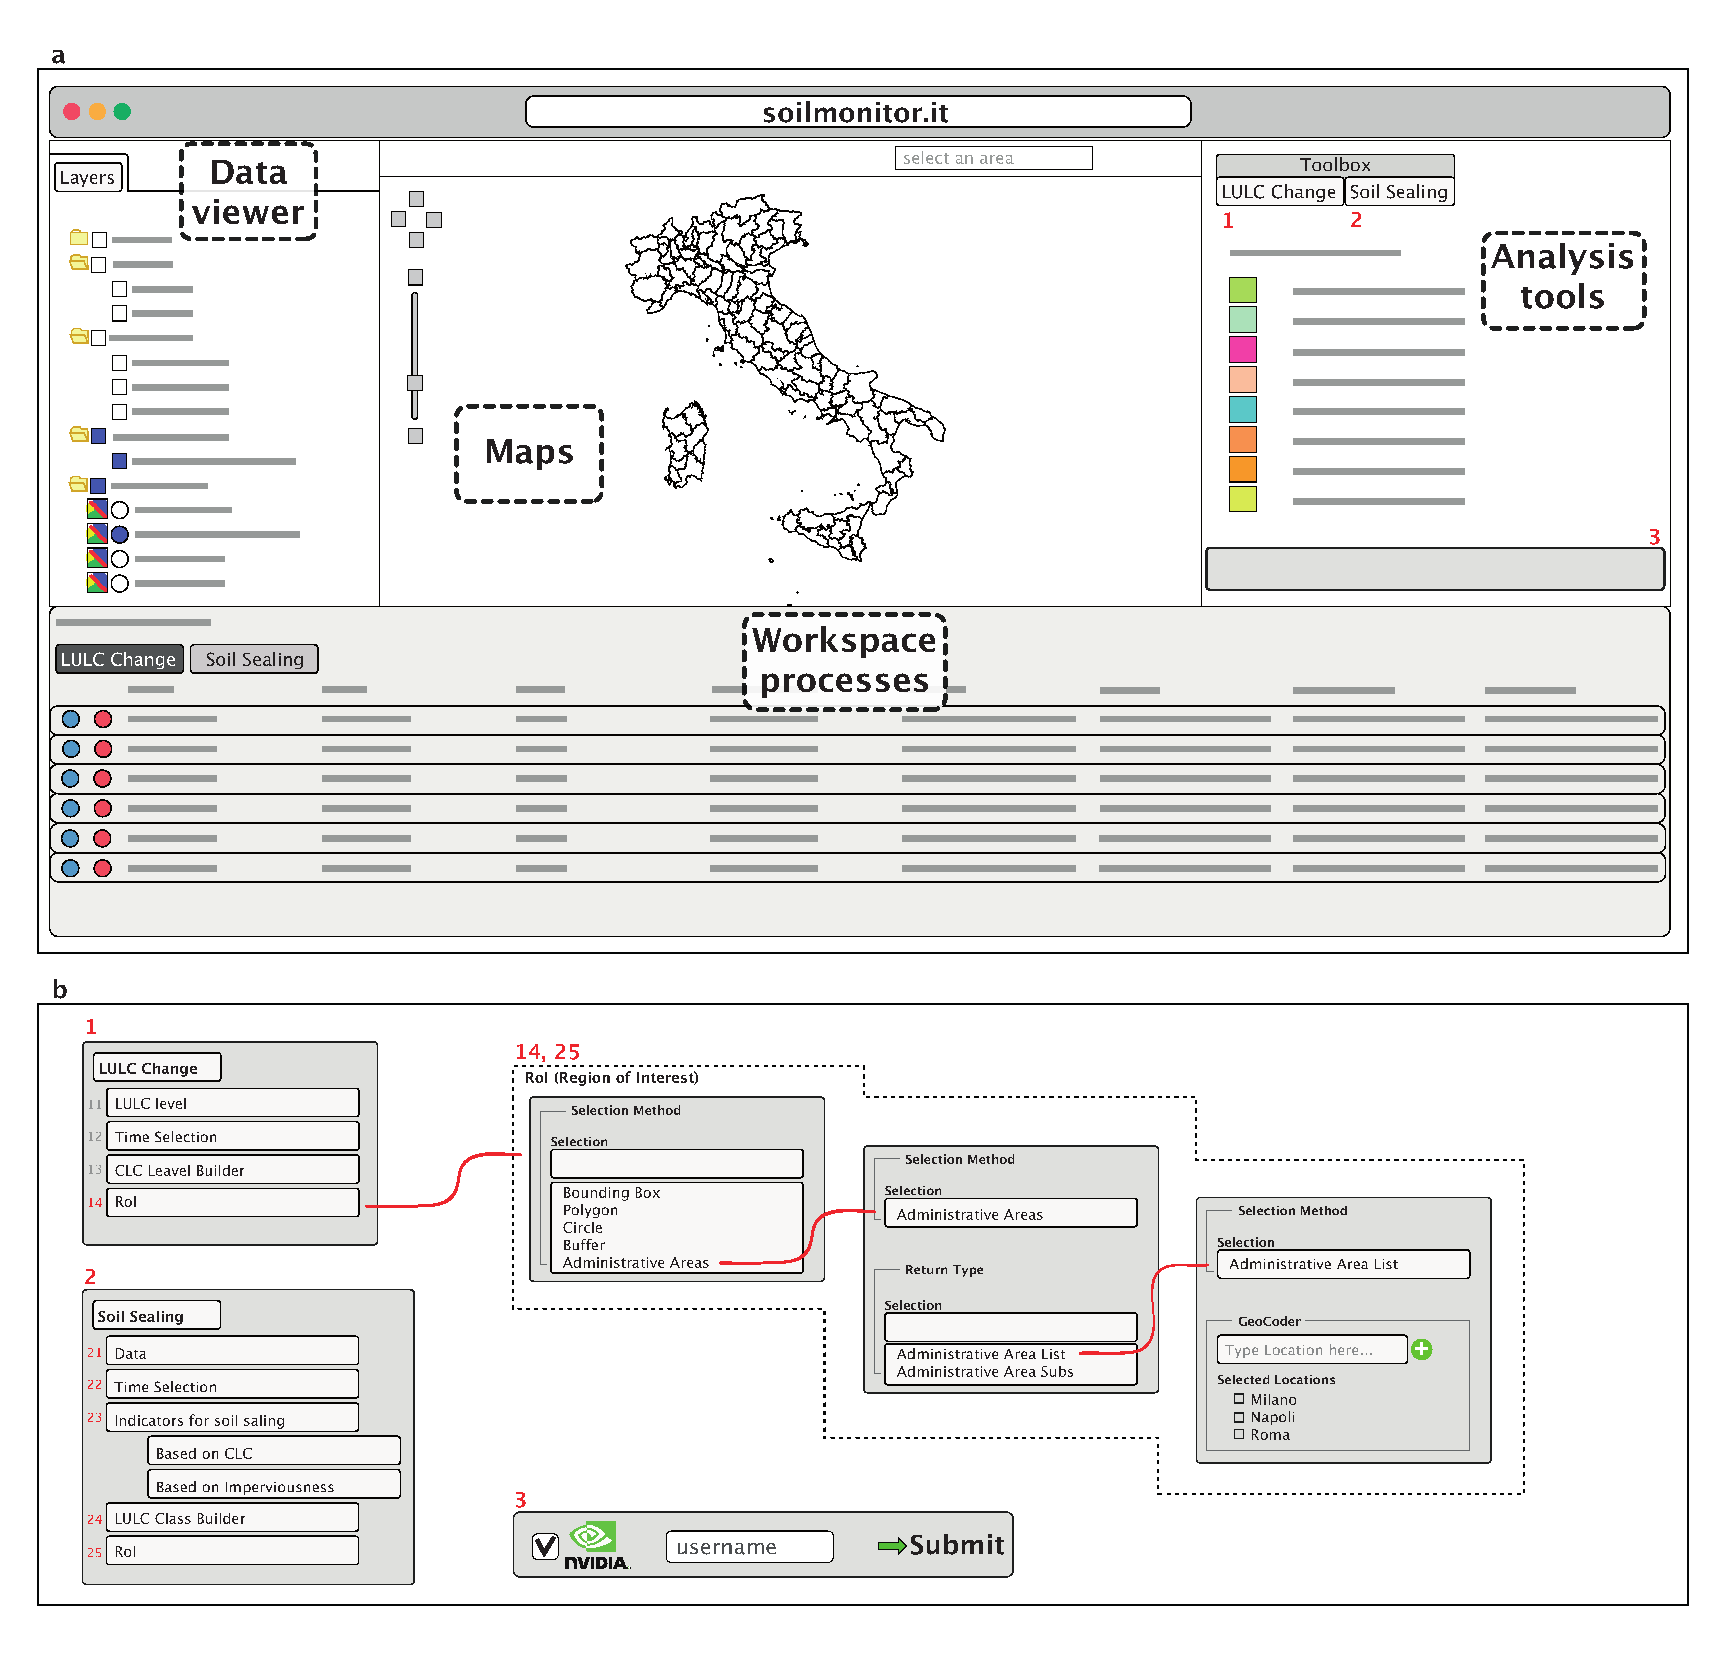
\includegraphics[width=500pt]{01_piattaforma.eps}}
    \DIFaddendFL \caption{\DIFdelbeginFL \DIFdelFL{Exemplification of the }\DIFdelendFL Soil Monitor \DIFaddbeginFL \DIFaddFL{web }\DIFaddendFL application\DIFaddbeginFL \DIFaddFL{.
             }\DIFaddendFL (\DIFdelbeginFL \DIFdelFL{SMapp}\DIFdelendFL \DIFaddbeginFL \DIFaddFL{a}\DIFaddendFL ) \DIFaddbeginFL \DIFaddFL{Exemplification of the }\DIFaddendFL dashboard with main panes (\DIFdelbeginFL \DIFdelFL{red }\DIFdelendFL \DIFaddbeginFL \DIFaddFL{back dashed }\DIFaddendFL boxes)\DIFaddbeginFL \DIFaddFL{, with reference to specific accordion panes (red annotations 1, 2, 3) described in (b)}\DIFaddendFL . 
             \DIFaddbeginFL \DIFaddFL{(b) }\DIFaddendFL The user can build a tailored query owing to the job submission steps \DIFaddbeginFL \DIFaddFL{(section \ref{sec:jobsubmission}) thanks to two distinct accordion panes}\DIFaddendFL , one \DIFaddbeginFL \DIFaddFL{designed }\DIFaddendFL for the LULC change \DIFdelbeginFL \DIFdelFL{toolbox }\DIFdelendFL \DIFaddbeginFL \DIFaddFL{analysis }\DIFaddendFL (\DIFdelbeginFL \DIFdelFL{a}\DIFdelendFL \DIFaddbeginFL \DIFaddFL{red 1}\DIFaddendFL ) and another one \DIFdelbeginFL \DIFdelFL{for }\DIFdelendFL \DIFaddbeginFL \DIFaddFL{dedicated to }\DIFaddendFL the soil sealing \DIFdelbeginFL \DIFdelFL{toolbox }\DIFdelendFL \DIFaddbeginFL \DIFaddFL{quantitative monitoring }\DIFaddendFL (\DIFdelbeginFL \DIFdelFL{b}\DIFdelendFL \DIFaddbeginFL \DIFaddFL{red 2}\DIFaddendFL ). \DIFaddbeginFL \DIFaddFL{A dedicated and advanced RoI building is available (red 14 and 25). }\DIFaddendFL Geospatial calculations can be distributed \DIFdelbeginFL \DIFdelFL{also }\DIFdelendFL on GPU cards owing to a tailored CUDA-C library \DIFdelbeginFL \DIFdelFL{developed for SMapp }\DIFdelendFL \DIFaddbeginFL \DIFaddFL{embedded in Soil Monitor }\DIFaddendFL (\DIFdelbeginFL \DIFdelFL{c}\DIFdelendFL \DIFaddbeginFL \DIFaddFL{red 3}\DIFaddendFL ).
             \DIFaddbeginFL \DIFaddFL{(LULC: Land Use and Land Cover; RoI: Region of Interest; CUDA: Compute Unified Device Architecture)
            }\DIFaddendFL } \label{fig:SMapp}
\end{figure}
\DIFdelbegin \DIFdel{SMapp is }\DIFdelend \DIFaddbegin \DIFadd{Soil Monitor is based on }\DIFaddend a three-tier logical architecture (Figure\ref{fig:GCI}) with separated processes made by 
(i) 
the \textit{\DIFdelbegin \DIFdel{visualization }\DIFdelend \DIFaddbegin \DIFadd{data }\DIFaddend tier\DIFdelbegin %DIFDELCMD < }%%%
\DIFdel{, which displays information related to the services, (ii)the }\textit{\DIFdel{logic tier}} %DIFAUXCMD
\DIFdel{that controls the functionality of the application by performing detailed processing, and (iii) the }\textit{\DIFdel{data tier}}%DIFAUXCMD
\DIFdelend \DIFaddbegin } \DIFadd{(section \ref{sec:dataTier})}\DIFaddend , which consists of the database where information is stored and retrieved in a manner that keeps data neutral and independent of the application servers and of the \DIFdelbegin \DIFdel{business logic }\DIFdelend \DIFaddbegin \DIFadd{logic tier,
(ii) the }\textit{\DIFadd{visualization tier}} \DIFadd{(section \ref{sec:viewTier}), which displays information related to the data and services
and 
(iii) 
the }\textit{\DIFadd{logic tier}} \DIFadd{that controls the functionality of the application by performing detailed geospatial processing (section \ref{sec:logicTier})}\DIFaddend .

\begin{figure}
[t] %DIF >  FIGURE 02
    % \includegraphics[width,,height=15pc,draft]
    % trim=left bottom right top, trim=0 0 0 50,clip,
%    \DIFdelbeginFL %DIFDELCMD < \centerline{\includegraphics[width=500pt]{Figure02.pdf}}
%%DIFDELCMD <     %%%
%%DIFDELCMD < \caption{%
%{%DIFAUXCMD
%\DIFdelFL{Main tiers, workflows, and technological components of the SMapp geospatial cyber infrastructure.}} %DIFAUXCMD
%\DIFdelendFL
\DIFaddbeginFL \centerline{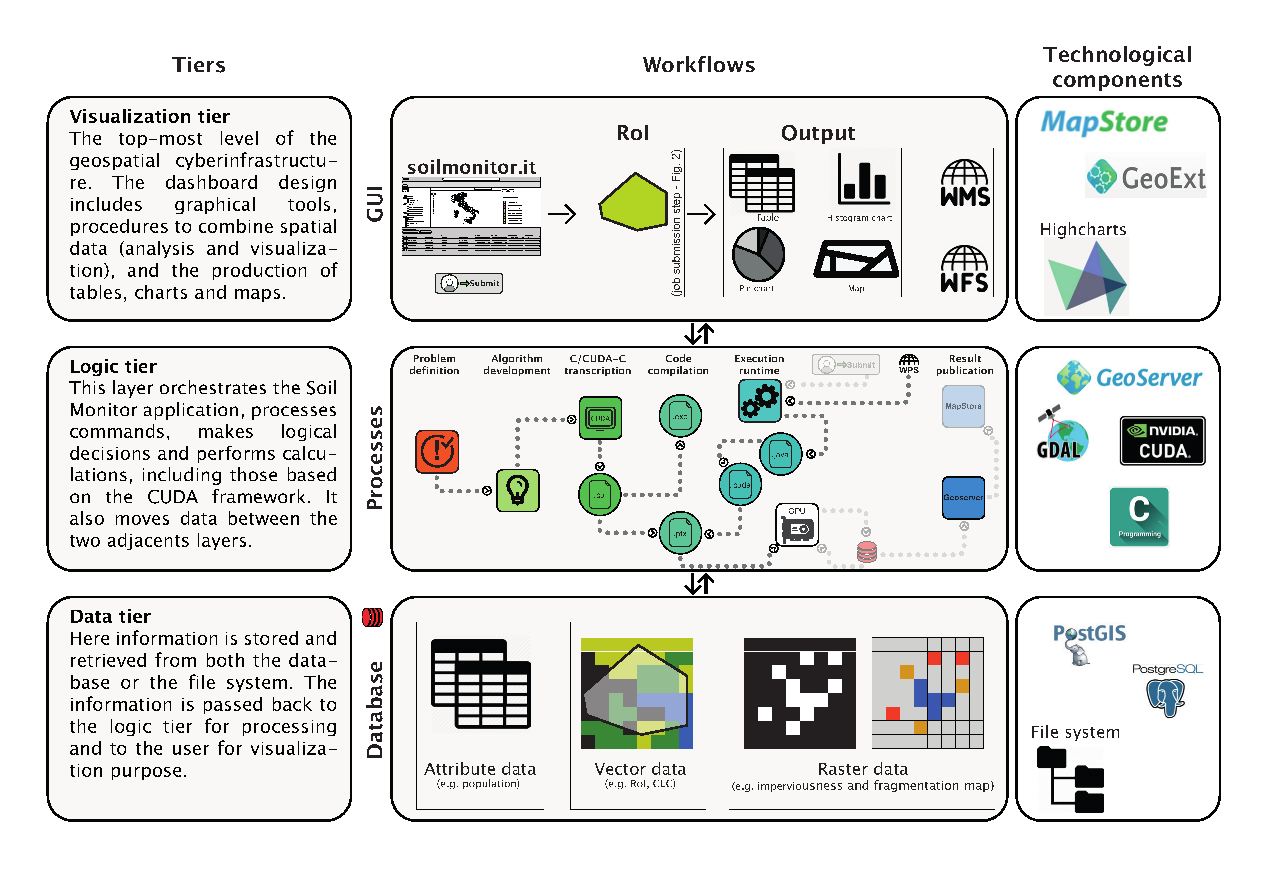
\includegraphics[width=500pt]{02_infrastruttura.eps}}
    \caption{\DIFaddFL{Main tiers, workflows, and technological components of the geospatial cyber-infrastructure behind Soil Monitor.
    The operating mode of the platform is sketched showing the flow of data that feeds different server functions (e.g. models), which, in turn, produces a set of services that can be finally accessed by the dashboard.
    (GUI: Graphical User Interface; RoI: Region of Interest)
    }} \DIFaddendFL \label{fig:GCI}
\end{figure}
\DIFdelbegin \DIFdel{In Figure \ref{fig:GCI},
a synthesis is sketched of the operating mode of the platform showing the flow of data that feed different server functions (e.g. models) , which, in turn, produce a set of services that can finally be accessed by the dashboard.
}\DIFdelend %DIF > The data and visualization tiers are described in section \ref{sec:dataTier} and section \ref{sec:viewTier} respectively, while a summary of the logic tier is in section \ref{sec:logicTier}.


\DIFdelbegin \subsection{\DIFdel{Workflow of the integrated platform}}
%DIFAUXCMD
\addtocounter{subsection}{-1}%DIFAUXCMD
\DIFdel{The integration of CUDA kernels, backend (i.e. Java and JCuda), and web interface requires a systematic workflow approach. 
A typical workflow includes three major steps: job submission, job status query, and results management, where the realization of each step requires integration across the three tiers of the cyberinfrastructure. 
}%DIFDELCMD < 

%DIFDELCMD < %%%
\DIFdel{Accordingly, Figure \ref{fig:SMapp} shows an overview of the available toolboxes for analysis, i.e. the toolbox for land use/land cover (LULC) change (Figure \ref{fig:SMapp}, a) and the toolbox for soil sealing indicators (Figure \ref{fig:SMapp}, b).
The user can build a tailored query owing to the two job submission steps, one for each toolbox. 
For any soil sealing indicator, the user must select --- according to the following hierarchical order --- the dataset they intend to use (i.e. CORINE land cover or high-resolution imperviousness layer, Figure \ref{fig:SMapp}, b1); the time of the analysis (one year or two years, Figure \ref{fig:SMapp}, b2); the selection of a soil sealing indicator (Figure \ref{fig:SMapp}, b3); the composition of LULC classes optionally (Figure \ref{fig:SMapp}, b4); and finally, the region of interest (Figure \ref{fig:SMapp}, b5) 
. Therefore, in order to ease the definition of a possible multi-polygon RoI, there is an ad hoc accordion pane for the rapid identification and selection of any Italian administrative unit.
The RoI definition accordion pane is particularly useful because it allows the user to select one or more administrative units at any level of the topological hierarchy (municipality, province, region)and to freely draw a new region of interest directly over the displayed map within SMapp.
For any subsequent query to the first one, the user can change only the parameters strictly required for the new job submission (e.g. change the indicator or the time) and SMapp will calculate the new indicator given the parameter set just defined. 
This behaviour was expressly required by end users to facilitate the instantiation of more requests for the purpose of scrutinizing the implementation of executed urban plans.
}%DIFDELCMD < 

%DIFDELCMD < %%%
\DIFdelend \subsection{Data \DIFdelbegin \DIFdel{layer}\DIFdelend \DIFaddbegin \DIFadd{(data tier) }\DIFaddend }
%DIF > \update{[materials]}}
\DIFaddbegin \label{sec:dataTier}
\DIFaddend The Open Geospatial Consortium\DIFdelbegin \DIFdel{(OGC)}\DIFdelend , which aims to develop community-consensus open geospatial standards, provides a family of enabling technologies for sharing geospatial data and analytical capabilities on a distributed network. 
Data sharing (interoperability) in Soil Monitor is supported both in input --- to visualize data coming from remote services (\DIFdelbegin \DIFdel{such as ISPRA }\DIFdelend \DIFaddbegin \DIFadd{e.g. those provided by ISPRA (Italian Institute for Environmental Protection and Research) }\DIFaddend or other national level administrative bodies) --- and in output to provide different data services such as WMS \DIFdelbegin \DIFdel{and WFS to allow a client visualization of static images for instance over the desktop computer in GIS environments.
Moreover, }\DIFdelend \DIFaddbegin \DIFadd{(Web Mapping Service, for serving georeferenced map images over the internet) and WFS (Web Feature Service, which supports the vector data model). %DIF >  to allow a client visualization of output images produced by the logic tier.
These }\DIFaddend web services are automatically appended to the \DIFdelbegin \DIFdel{new GIS data calculated by the CUDA engine }\DIFdelend \DIFaddbegin \DIFadd{output images produced by the logic tier %DIF > new geospatial data %calculated by the CUDA engine 
}\DIFaddend to enable the visualization of results both locally within Soil Monitor, and remotely, for instance, within desktop GIS software environments.
Indeed, after ingestion in GeoServer, data become available for visualization and calculation purposes for the whole Italian territory Soil Monitor stores as follows:
 \begin{itemize} 
    \item The \DIFdelbegin \DIFdel{land use and land cover }\DIFdelend \DIFaddbegin \DIFadd{Land Use and Land Cover (LULC) }\DIFaddend map in the period of 1956-60 produced by the Italian Touring Club in collaboration with National Council of Research, CNR (map of land use in Italy, scale 1: 200.000).
    \item The CORINE Land Cover (CLC) is a valuable source of information about land use and land cover, produced at the European level since the '90s and updated regularly (originally coordinated by the European Commission and the European Environmental Agency; now included in the Copernicus framework).
    CLC vector data are produced by photointerpretation of satellite images, with a minimum mapping unit of 25 ha and a classification system organized in three \DIFaddbegin \DIFadd{hierarchical }\DIFaddend levels of thematic detail: level 1 with 5 land use and land cover classes, level 2 with 15 land use and land cover classes, and level 3 with 43 land use and land cover classes. 
    In \DIFdelbegin \DIFdel{SMapp}\DIFdelend \DIFaddbegin \DIFadd{Soil Monitor}\DIFaddend , the raster version of CLC with a spatial resolution of 100 m is available for the years 1990, 2000, 2006, 2012, and 2018. Considering the homogeneity over the entire Europe and the constant update, CLC is largely used for spatial analysis, land cover change assessment, and policy making.
    \item The National High-Resolution Soil Consumption (NHRSC) \DIFaddbegin \DIFadd{dataset }\DIFaddend was produced for Italy by ISPRA (ISPRA, 2016); the NHRSC is a raster that identifies artificial land cover areas with a spatial resolution of 10 m, produced for 2006, 2009, 2012, 2015, 2016, 2017 and 2018 with a semi-automatic classification of satellite images and the integration of local ancillary data such as OpenStreetMap; NHRSC included in Soil Monitor has a binary classification system such as non-sealed soil and sealed soil, according to the description given in Table \ref{tab:IMPclasses}.
    \item The administrative units: Italian administrative data are provided by the \DIFdelbegin \DIFdel{national }\DIFdelend \DIFaddbegin \DIFadd{Italian }\DIFaddend institute of statistics (ISTAT). 
    These data represent the administrative units (also NUTS) in vector format.
    \item The population: population data are provided at the Municipal level by ISTAT, which periodically collects census data and updates this information every year. 
    \item The digital soil grids: Predictions on key soil properties performed globally at 250 m spatial resolution by ISRIC\footnote{available at http://data.isric.org/geoserver/sg250m/wms}. This is an example of \DIFaddbegin \DIFadd{Open Geospatial Consortium compliant }\DIFaddend interoperability based on \DIFdelbegin \DIFdel{the OGC standard called Web Mapping Service (WMS )}\DIFdelend \DIFaddbegin \DIFadd{WMS which is used as input source of georederenced map images in Soil Monitor}\DIFaddend .
 \end{itemize} 
\begin{table}
\caption{Legend \DIFaddbeginFL \DIFaddFL{and classes }\DIFaddendFL of the \DIFdelbeginFL \DIFdelFL{NHRSC map}\DIFdelendFL \DIFaddbeginFL \DIFaddFL{National High-Resolution Soil Consumption dataset}\DIFaddendFL }\label{tab:IMPclasses}
\centering
\begin{tabular}[t]{ l l | l } 
\hline
\textbf{Code} & \textbf{Description} & \textbf{Classes} \\
\hline
\multirow{9}{4em}{0} & \multirow{9}{10em}{Non-sealed soil} & Tree/shrubs \\ 
 &  & Crops \\ 
 &  & Grassland \\ 
 &  & Water bodies \\ 
 &  & Wetlands \\ 
 &  & Rocks, beaches, and dunes \\ 
 &  & Glaciers and perpetual snow \\ 
 &  & Sport areas (pervious surface) \\ 
 &  & Other pervious surfaces \\ 
\hline
\multirow{10}{4em}{1} & \multirow{10}{10em}{Sealed soil} & Buildings \\ 
 &  & Road/Squares/Parking \\ 
 &  & Railway sites \\ 
 &  & Airports and ports (impervious surfaces) \\ 
 &  & Impermeable areas in sports fields \\ 
 &  & Permanent greenhouses \\ 
 &  & Solar farms on land \\ 
 &  & Mining areas \\ 
 &  & Dump sites \\ 
 &  & Other impervious areas \\
\hline
2 & Unclassified & \\
\hline
3 & Area outside the national boundary & \\
\hline
\end{tabular}
\end{table}
The CLC and Touring layers have been rasterized into \DIFaddbegin \DIFadd{images at }\DIFaddend 8-bit \DIFaddbegin \DIFadd{and }\DIFaddend 100 meters resolution \DIFdelbegin \DIFdel{images }\DIFdelend to enable the grid-based calculations\DIFdelbegin \DIFdel{based on the CUDA framework. }\DIFdelend \DIFaddbegin \DIFadd{. %DIF >  based on the CUDA framework.
}\DIFaddend Comparisons between CLC layers can be executed at three different levels of the legend detail (Level 1, Level 2, and Level 3) having different numbers of land use and land cover classes. 
In order to enable \DIFdelbegin \DIFdel{comparison }\DIFdelend \DIFaddbegin \DIFadd{comparisons }\DIFaddend with the Italian Touring Club layer, the most detailed CORINE legend (Level 3) has been homogenized with that from Touring Club. 
The imperviousness layers have been binarized (2-bit images) by applying a threshold to the level of imperviousness equal to 30\% \DIFaddbegin \DIFadd{of the pixel area}\DIFaddend , above which a pixel is taken as \DIFdelbegin \DIFdel{impervious}\DIFdelend \DIFaddbegin \DIFadd{sealed}\DIFaddend .

\subsection{\DIFdelbegin \DIFdel{Visualization layer}\DIFdelend \DIFaddbegin \DIFadd{Development of the dashboard (visualization tier) }\DIFaddend }
%DIF > \update{[methods]}}
\DIFaddbegin \label{sec:viewTier}
%DIF >  Visualization of data and use of soil sealing tools
\DIFaddend The dashboard design includes graphical tools, procedures to combine spatial data (analysis and visualization), and the production of tables and maps. 
The frontend application is based on MapStore (Figure \ref{fig:GCI}) and the overall structure of the graphical user interface can be distinguished in four main panes: the data, the map, the workspace, and the \DIFdelbegin \DIFdel{accordion }\DIFdelend \DIFaddbegin \DIFadd{analysis }\DIFaddend panes (Figure \ref{fig:SMapp}\DIFaddbegin \DIFadd{a, dashed boxes}\DIFaddend ).
The \textit{data pane} enables the visualization of different data, but not all information used in the calculation is visible, such as the population vector data. 
Moreover, MapStore enables users to add external data sources equipped with web services for rendering rasters and vectors, enhancing the overall interoperability of the platform. 
For instance, it can be particularly useful to compare the result of calculations with constraint maps coming from other data providers, such as the Italian Ministry of Cultural and Environmental Heritage, to check the soil sealing results. Furthermore, the \textit{map pane} enables the visualization of both the input geospatial data and the output maps calculated by the models and indicators available in the toolboxes. 
Moreover, the \textit{workspace pane} is where all instantiated requests are displayed. 
The toolboxes enable the allocation of several asynchronous requests per single user at the same time, which means that they can be calculated concurrently on the available CPU and GPU resources. 
The processes launched by users, which may be running at the same time, are displayed in the workspace as running, completed or interrupted according to their states. 
The \DIFaddbegin \textit{\DIFadd{analysis pane}} \DIFadd{is made by two dedicated }\DIFaddend \textit{accordion panes} \DIFdelbegin \DIFdel{are used }\DIFdelend \DIFaddbegin \DIFadd{(Figure \ref{fig:SMapp}b, red annotations 1 and 2) that are available }\DIFaddend to give the user full access to the \DIFdelbegin \DIFdel{processing layer }\DIFdelend \DIFaddbegin \DIFadd{logic tier }\DIFaddend parameters in a transparent way\DIFdelbegin \DIFdel{(see Figure \ref{fig:SMapp} for the query building procedure)}\DIFdelend .

In addition to standard open-source codes available from the dual infrastructure GeoServer and MapStore, \DIFdelbegin \DIFdel{additional }\DIFdelend \DIFaddbegin \DIFadd{new }\DIFaddend codes have been written to enrich \DIFdelbegin \DIFdel{functionality}\DIFdelend \DIFaddbegin \DIFadd{the functionality of Soil Monitor}\DIFaddend .
For example, the client side has a dedicated interface to \DIFdelbegin \DIFdel{configure the RoI , which includes different methods such as the multiple selection of several administrative units at any hierarchical level (municipalities, provinces, and regions) . 
Another example is given by }\DIFdelend \DIFaddbegin \DIFadd{build a customized RoI (more details provided in the job submission, section \ref{sec:jobsubmission}) and }\DIFaddend the availability of different types of \DIFaddbegin \DIFadd{Highcharts }\DIFaddend plots that are generated dynamically in addition to the \DIFdelbegin \DIFdel{geodata }\DIFdelend \DIFaddbegin \DIFadd{visualization of map images, }\DIFaddend in order to enhance the readiness and interpretation of results.

\subsection{\DIFdelbegin \DIFdel{Processing layer}\DIFdelend \DIFaddbegin \DIFadd{Soil sealing metrics embedded in Soil Monitor }\DIFaddend } \DIFdelbegin \DIFdel{On the server side, specific classes written in Java and CUDA have been developed to perform the calculations required to account for soil sealing and land take. 
Some calculations may be very demanding since they rely on high resolution grids (i.e. a square pixel of size 20 m) or on high thematic detail (i.e. CLC Level 3) feeding requests over large geographical areas (such as administrative regions or the whole Italy). For instance, this is the case of the rural fragmentation index, which is computed on the 20 m imperviousness layers. 
Even when selecting a small RoI, the relative high calculation demand depends on the logic of the algorithm itself, since it has to visit more than six thousand neighbour pixels $\left( \sim ( 800/\left(20\times2\right) )^2 \right)$ to calculate how fragmented each target pixel is, given a radius of 800 meters in the moving window selected by the user.
These cases may not manage to return answers in real-time or near-real-time for relatively large geographical extents, which explains one of the reasons why calculations are instantiated asynchronously.
}%DIFDELCMD < 

%DIFDELCMD < %%%
\DIFdel{In addition to data services, Soil Monitor implements Web Processing Services (WPS), which expose the algorithm of a soil sealing model or indicator outside the web application (Fig. 2). 
This was particularly useful to perform tests about the goodness of calculations in different spatial and temporal contexts, without the tedious infilling of the accordion panes to submit more and more requests. 
The test was performed by invoking a geospatial process with a known set of parameters by means of the supported POST request method submitted directly to the GeoServer endpoint. 
Subsequently, the parameters are passed to JCUDA, which, in turn, invokes the execution of CUDA kernels compiled in PTX files. 
The POST requests can be submitted from within the Unix terminal and, in our work, from MatLab scripts specifically designed for testing purposes. 
The testing procedure collects the results coming from the three independent computing environments: 
(i) the stand-alone executable (EXE) compiled from the source CUDA-C code; 
(ii) the WPS based on the JAI-JCUDA-CUDA chain executing the PTX compiled from the same source code used in the previous point; and 
(iii) a MatLab code implementing an alternative algorithm to perform the same geospatial processing. 
The test ends with a comparison of results coming from the three approaches to check for both speed performance and accuracy. 
This procedure was used as a standard during the development stage in order to test for inaccuracies in either the CUDA algorithms targeted to geospatial processing or in the deployment of the computing chains.
Further, WPS can be easily adapted to enable the dynamic binding of geospatial processes to aid client needs, such as running a standardized algorithm on personal data.
}%DIFDELCMD < 

%DIFDELCMD < %%%
\DIFdel{The CUDA framework and its binding from Java is implemented in the processing layer, where a list of developed CUDA kernels are loaded as a library in the infrastructure. 
First, a library of CUDA kernels is written in C, which can be used both standalone and as a compilation in PTX. 
Further, the Parallel Thread Execution (PTX) is a low-level parallel thread execution virtual machine and instruction set architecture, which provides a stable programming model and instruction set for general purpose parallel programming. 
Moreover, the PTX instructions are optimized for and translated to native target-architecture instructions. 
Second, the very fundamental CUDA kernels compiled as PTX files work as primitives that are combined in the JCUDA layer to build the crafted algorithms to address the soil sealing geospatial calculations. 
The advantage of this type of orchestration is that new models and indicators that may be added in the Soil Monitor toolboxes can be implemented using the same library of CUDA kernels, while little development and coding is required.
Accordingly, an example of the pyramidal architecture based on the CUDA kernels is presented in Figure\ref{fig:ccl}, describing the calculation of the discontinuous urban fabric surface ($S_{DUF}$) using a connected component labelling algorithm specifically developed for SMapp. 
This algorithm is made of 8 CUDA kernels and one thousand lines of code performing the labelling of a 2-bit high resolution impervious layer in a 64-bit layer of ordered labels, one for each distinct urban patch.
Consequently, after identification and labelling, urban patches are sorted and then a threshold (90\%) is applied to extract only patches belonging to the discontinuous urban fabric. 
These patches are summed up to calculate the overall discontinuous urban fabric surface.
}%DIFDELCMD < 

%%DIFDELCMD < 
%\begin{figure}
%[t]
%%DIFDELCMD <     %%%
%%DIF <  \includegraphics[width,,height=15pc,draft]
%    %DIFDELCMD < \centerline{\includegraphics[width=500pt]{Figure03.pdf}}
%%DIFDELCMD <     %%%
%%DIFDELCMD < \caption{%
%{%DIFAUXCMD
%\DIFdelFL{The $S_{DUF}$ calculation developed in the CUDA framework within Soil Monitor GCI. 
%    The pixel-based elaboration is solved by a connected component labelling algorithm written in CUDA-C. 
%    Elapsed times in the kernel box refer to an image of size $180 \times 10^6$ pixels.}} %DIFAUXCMD
%%DIFDELCMD < %DIFDELCMD < \label{fig:ccl}%%%
%%DIFDELCMD < 
%\end{figure}
%%DIFDELCMD < 

%DIFDELCMD < %%%
\section{\DIFdel{Description of models/indicators of soil sealing}}
%DIFAUXCMD
\addtocounter{section}{-1}%DIFAUXCMD
\DIFdel{The }\DIFdelend %DIF > \update{[methods]}}
\DIFaddbegin \label{sec:metrics}
\DIFadd{Huge amount of metrics is available to monitor and measure urban growth, urban density and sprawl, soil sealing and land take.
The limited }\DIFaddend list of indicators \DIFdelbegin \DIFdel{we have }\DIFdelend developed and implemented \DIFdelbegin \DIFdel{are given in Table 2, which }\DIFdelend \DIFaddbegin \DIFadd{in Soil Monitor }\DIFaddend have been chosen in close collaboration with \DIFaddbegin \DIFadd{italian }\DIFaddend urban planners to address their \DIFdelbegin \DIFdel{planning needs . 
They refer to land use /land cover descriptors}\DIFdelend \DIFaddbegin \DIFadd{specific needs while avoiding redundancy of information often given by similar metrics. 
A summary of available metrics is given in Table \ref{tab:SMappToolbox}.
They include land use and land cover metrics}\DIFaddend , rate of change of land use \DIFdelbegin \DIFdel{/}\DIFdelend \DIFaddbegin \DIFadd{and }\DIFaddend land cover, marginal soil sealing, extent of urban sprawl, density of urban boundaries, degree of urban dispersion, rural \DIFdelbegin \DIFdel{/}\DIFdelend \DIFaddbegin \DIFadd{and }\DIFaddend urban fragmentation, \DIFdelbegin \DIFdel{global }\DIFdelend land take dynamics, and estimate of loss in food supply due to \DIFdelbegin \DIFdel{soil sealing. 
The table refers to }\DIFdelend \DIFaddbegin \DIFadd{land take. 
}

\DIFadd{The metrics shown in Table \ref{tab:SMappToolbox} can use as input one of }\DIFaddend the two official datasets described \DIFdelbegin \DIFdel{above, i.e. the Corine Land Cover and the }\DIFdelend \DIFaddbegin \DIFadd{in the data tier section above, that is a grid of LULC or a grid of }\DIFaddend soil imperviousness. 
The \DIFdelbegin \DIFdel{CLC }\DIFdelend \DIFaddbegin \DIFadd{LULC }\DIFaddend layers allow investigations on multiple classes of land use and land cover but at a relatively coarser spatial resolution (either 100 m or 250 m spatial resolution \DIFaddbegin \DIFadd{with the CLC or Touring Club data, respectively}\DIFaddend ).
Conversely, soil imperviousness is available over high spatial detailed layers (20 m spatial resolution) \DIFdelbegin \DIFdel{and }\DIFdelend \DIFaddbegin \DIFadd{but }\DIFaddend aggregates the information of land use in only two classes, \DIFdelbegin \DIFdel{i.e. }\DIFdelend \DIFaddbegin \DIFadd{that is }\DIFaddend sealed and unsealed land \DIFdelbegin \DIFdel{. 
Furthermore}\DIFdelend \DIFaddbegin \DIFadd{as defined in Table \ref{tab:IMPclasses}. 
Finally}\DIFaddend , the choice between the two datasets reflects the kind of soil sealing \DIFdelbegin \DIFdel{indicator}\DIFdelend \DIFaddbegin \DIFadd{metric}\DIFaddend , the detail in the thematic domain, and the spatial resolution required in the output map.

\begin{table}
[b]
    \caption{ \DIFdelbeginFL \DIFdelFL{Models }\DIFdelendFL \DIFaddbeginFL \DIFaddFL{Metrics implemented }\DIFaddendFL in \DIFdelbeginFL \DIFdelFL{SMapp toolbox }\DIFdelendFL \DIFaddbeginFL \DIFaddFL{Soil Monitor }\DIFaddendFL for soil sealing and land take. }
    \label{tab:SMappToolbox}
    \small
    \centering
    \begin{tabular}{m{0.3cm} p{0.1cm} p{1.2cm} p{3.5cm} *{3}{p{2.7cm}} p{1.0cm} }

    \toprule
        & \textbf{ID} & \textbf{Model} & \textbf{Formula$^\dagger$} & \textbf{Description} & \textbf{Application} & \textbf{Techonological Novelty} & \textbf{Outputs}\\
    \midrule\midrule

    \multirow{5}{*}{ \rotatebox[origin=c]{90}{ \shortstack[c]{ Calculation using LULC rasters at 100m spatial resolution \\ (e.g. CLC produced by Copernicus)} } } 
    & 0 & LULC & --- & Change of state of each LULC class from a reference year to a current year & Evolutionary \DIFdelbeginFL \DIFdelFL{traiectories }\DIFdelendFL \DIFaddbeginFL \DIFaddFL{trajectories }\DIFaddendFL & CUDA kernels producing both an interactive change matrix and a map of all changes & pie chart, \DIFdelbeginFL \DIFdelFL{vector }\DIFdelendFL \DIFaddbeginFL \DIFaddFL{raster }\DIFaddendFL map  \\

    & 1	& Coverage Coefficient & $\frac{S_{CLC_i}}{S_{AU}}$ & Fraction of total surface covered by i-th land use/cover class & Classes consistency within a user defined RoI (admin unit or free area) & None & bar chart, vector map \\

    & 2 & Rate of Change & 
    $\frac{ \left(S_{CLC_i}\right)_{T_2} - \left(S_{CLC_i}\right)_{T_1} }{ \left(S_{CLC_i}\right)_{T_1} }$ 
    & Rate of change of any i-th land use/cover class & Change of classes consistency within a user defined RoI (admin unit or free area) & None & bar chart, vector map \\

    & 3 & Marginal Land Take & 
    $\frac{ \left(S_{CLC_1}\right)_{T_2} - \left(S_{CLC_1}\right)_{T_1} }{ \left(POP_{au}\right)_{T_2} - \left(POP_{au}\right)_{T_1} }$
    & Ratio between urbanization variation and population growth variation between two years & Analyse variation of urbanization with respect to variation of population to depict temporal trends & None & bar chart, vector map \\

    & 4	& Urban Sprawl & 
    $\frac{ \frac{ \left(S_{CLC_1}\right)_{T_2} - \left(S_{CLC_1}\right)_{T_1} }{ \left(S_{CLC_1}\right)_{T_1} }  }     { \frac{ \left(POP_{au}\right)_{T_2} - \left(POP_{au}\right)_{T_1} }{ \left(POP_{au}\right)_{T_1} } }$
    & Ratio between urbanization rate and population growth rate between two years & Standardized version of marginal land take & None & bar chart, vector map \\

    \midrule

    \multirow{9}{*}{ \rotatebox[origin=c]{90}{ \shortstack[c]{Calculation using high resolution imperviousness rasters at 20m spatial resolution \\ (NHRSC produced by ISPRA)} } } 
    & 5 & Urban sprawl & 
    $\frac{S_{DUF}}{S_{UT}}$ 
    & Ratio between discontinuous urban fabric and total urban surface & To know the composition of urban development related to sprawl phenomenon, which can be related to fragmentation & Tailored connected component \DIFdelbeginFL \DIFdelFL{labeling }\DIFdelendFL \DIFaddbeginFL \DIFaddFL{labelling }\DIFaddendFL algorithm in CUDA & bar chart \\

    & 6 & Edge Density (ED) &
    $\frac{P_{UT}}{S_{UT}}$ 
    & Ratio between perimeter and surface of urbanized ares in selected RoI & Density of urban margins, which is related to urban fragmentation & CUDA kernels computing both the perimeter and the urbanized area & bar chart \\

    & 7 & Urban Area &
    $\frac{S_{UT}}{S_{AU}}$ 
    & Fraction of total surface covered by urbanization & To know the magnitude of land take related to the administrative unit & CUDA kernels computing the urbanized area	& \DIFdelbeginFL \DIFdelFL{barchart }\DIFdelendFL \DIFaddbeginFL \DIFaddFL{bar chart }\DIFaddendFL \\

    & 8	& Largest Class Patch Index (LCPI) & 
    $\frac{S_{max}}{S_{UT}}$ 
    & Fraction of urban surface within the largest urban patch & Represents the level of compactness of the urban area & CUDA kernels computing the connected component \DIFdelbeginFL \DIFdelFL{labeling	}\DIFdelendFL \DIFaddbeginFL \DIFaddFL{labelling	}\DIFaddendFL & bar chart \\

    & 9	& Residual Mean Patch Surface (RMPS) &
    $\frac{S_{DUF}}{N_{DUF}}$ 
    & Average surface of all urban patches excluding the largest patch & Mean patch area within the discontinuous urban fabric, which can be related to urban texture & CUDA kernels computing the connected component \DIFdelbeginFL \DIFdelFL{labeling }\DIFdelendFL \DIFaddbeginFL \DIFaddFL{labelling }\DIFaddendFL & bar chart \\

    & 10 & Rural/Urban Fragmentation &
    \DIFdelbeginFL \DIFdelFL{$\frac{\sum^{N}_{k=1} V_k}{ n-1 }$ 
    }\DIFdelendFL \DIFaddbeginFL \DIFaddFL{$\frac{\sum^{N}_{k=1} V_k}{ N-1 }$ 
    }\DIFaddendFL & Fraction of pixels having the same value of the \DIFdelbeginFL \DIFdelFL{center }\DIFdelendFL \DIFaddbeginFL \DIFaddFL{centre }\DIFaddendFL pixel in a mask & e.g. on rural \DIFdelbeginFL \DIFdelFL{center }\DIFdelendFL \DIFaddbeginFL \DIFaddFL{centre }\DIFaddendFL pixels it highlights ecological corridors & 1k lines of code; 6 CUDA kernels; 8 geospatial parameters & raster map \\

    & 11 & Land Take (and Gains) &
    $ \left( V_{pix} \right)_{T_2} - \left( V_{pix} \right)_{T_1}$ 
    & Difference of the value of a pixel between two \DIFdelbeginFL \DIFdelFL{differenr }\DIFdelendFL \DIFaddbeginFL \DIFaddFL{different }\DIFaddendFL times & A map with three possible pixel values: (0) if no change \DIFdelbeginFL \DIFdelFL{occured}\DIFdelendFL \DIFaddbeginFL \DIFaddFL{occurred}\DIFaddendFL ; (-1) if land take; (+1) if land gain & Based on the basic reduce CUDA kernel & raster map, bar chart \\

    & 12 & Net Loss of Food Supply &
    $ \sum_{pix=0}^{image} \left( \left( V_{pix} \right)_{T_2} - \left( V_{pix} \right)_{T_1} \right) \times C $ 
    & --- & Potential loss of aggregated ecosystem function (coeff :: FAO) & Based on the basic reduce CUDA kernel & bar chart \\

    & 13 & Model of Urban Development & Composite of IDs 6, 8 and 9 & --- & ---	& Same as aggregating IDs 6, 8 and 9 plus a 3-D view highlighting urban development in both different administrative units and times & 3-D \DIFdelbeginFL \DIFdelFL{scatplot }\DIFdelendFL \DIFaddbeginFL \DIFaddFL{scatter plot }\DIFaddendFL \\

    \midrule\bottomrule

    \multicolumn{8}{p{17.2cm}} % 13.9cm is the sum of all column previously defined by p{}
    {
      \DIFdelbeginFL %DIFDELCMD < \footnotesize{$^\dagger$Definitions. 
%DIFDELCMD <       $S$:area;
%DIFDELCMD <       $P$:perimeter;
%DIFDELCMD <       $V$:value;
%DIFDELCMD <       $S_{CLC_i}$:area of $i_{th}$ CORINE Land Cover class at selected legend level; 
%DIFDELCMD <       $S_{AU}$: area of administrative unit; 
%DIFDELCMD <       $S_{CLC_1}$: area of urban CLC class at selected legend level; 
%DIFDELCMD <       AU: administrative unit (city, province, region, \ldots); 
%DIFDELCMD <       $T_1$: time before; 
%DIFDELCMD <       $T_2$: time after; 
%DIFDELCMD <       $POP_{AU}$: population within AU; 
%DIFDELCMD <       $S_{DUF}$: area of discontinuous urban fabric; 
%DIFDELCMD <       $N_{DUF}$: number of urban patches within discontinuous urban fabric; 
%DIFDELCMD <       $S_{UT}$: total urban area; 
%DIFDELCMD <       $V_k$: value of the pixel \textit{k} within the kernel of N pixels }%%%
\DIFdelendFL \DIFaddbeginFL \footnotesize{$^\dagger$Definitions. 
      $S$:area;
      $P$:perimeter;
      $V$:value;
      $S_{CLC_i}$:area of $i_{th}$ CORINE Land Cover class at selected legend level; 
      $S_{AU}$: area of administrative unit; 
      $S_{CLC_1}$: area of urban CLC class at selected legend level; 
      AU: administrative unit (city, province, region, \ldots); 
      $T_1$: time before; 
      $T_2$: time after; 
      $POP_{AU}$: population within AU; 
      $S_{DUF}$: area of discontinuous urban fabric; 
      $N_{DUF}$: number of urban patches within discontinuous urban fabric; 
      $S_{UT}$: total urban area; 
      $V_k$: amount of fragmentation of the target pixel \textit{k} within the moving window of N pixels }\DIFaddendFL ;
      $V_{pix}$:value of pixel in NHRSC raster;
      C: FAO coefficient equal to 0.6 $persons \times ha^{-1} \times year^{-1}$
      .
    }
    \end{tabular}
\end{table}
\DIFdelbegin \section{\DIFdel{Application: case studies with validation}}
%DIFAUXCMD
\addtocounter{section}{-1}%DIFAUXCMD
\subsection{\DIFdel{The case study of Italy}}
%DIFAUXCMD
\addtocounter{subsection}{-1}%DIFAUXCMD
\DIFdel{In }\DIFdelend \DIFaddbegin \subsubsection{ \DIFadd{Soil sealing metrics operational: the fast geoprocessing engine (logic tier) }} %DIF >  \update{[methods]} }
\label{sec:logicTier}
%DIF > \update{We need a description of the logic tier avoiding it being viewed as a technical report/manual}\\
\DIFadd{On the server side, specific functions written in Java (classes) and CUDA (kernels) have been developed to perform the calculations required by the metrics reported in Table \ref{tab:SMappToolbox}. 
Some calculations may be very demanding since they rely on high resolution grids (i.e. a square pixel of size 20 m) or on high thematic detail (i.e. CORINE land cover at level 3 with 43 classes) feeding requests over large geographical areas (such as administrative regions or the whole Italy).
These cases may not manage to return answers in real-time or near-real-time
%DIF > for relatively large geographical extents
, which explains why 
(i) calculations are instantiated asynchronously in the geospatial cyber-infrastructure, and
(ii) metrics are implemented in GPU computing using the CUDA framework by NVIDIA.
The asynchronous instantiation of calculations in the cyber-infrastructure means that a a request can be submitted without waiting for previous ones to be finished.
This allows both the multi-user concurrency and the submission of as many requests as needed by a single user to address own analysis.
The user can close the web page and then navigate back to the Soil Monitor workspace to find the results ready for visualization and interpretation.
}

\DIFadd{The second characteristic of the geoprocessing engine is the implementation of most of the metrics showed in Table \ref{tab:SMappToolbox} by means of the CUDA-C programming language.
The CUDA code and its binding from Java is implemented in the logic tier in which %DIF > is connected to the data tier and the visualization tier.
%DIF > In the logic tier a 
the list of developed CUDA kernels is loaded as a library in the infrastructure.
The development of the fast geoprocessing engine is as follows (see the workflow in logic tier of Figure \ref{fig:GCI}).
First, a library of CUDA kernels is written in C and then compiled in PTX. 
Second, the most fundamental CUDA kernels work as primitives that are assembled in the JCUDA layer to build the crafted algorithms  addressing the calculation of soil sealing metrics.
This is referenced as the Java/JCUDA/CUDA pipeline of Soil Monitor.%DIF >  which is a novelty in the implementation of spatial decision support systems using WebGIS over the internet.
}

\DIFadd{In addition to data services (section \ref{sec:dataTier}), Soil Monitor implements Web Processing Services (WPS) which expose algorithm of soil sealing metrics outside the web application (Figure \ref{fig:GCI}, logic tier). 
WPS allows to invoke a geospatial process with a known set of parameters by means of the supported POST request method (using the XML language) submitted directly to the GeoServer endpoint (JAVA layer).
After the submission of the request using either the Soil Monitor graphical interface or the POST method, the parameters are passed to the JCUDA layer, which, as a software bridge, invokes the execution of the CUDA kernels compiled in PTX files.
This is recognized as the }\textit{\DIFadd{forward}} \DIFadd{high performance computing phase of the geoprocessing engine, which spans from the request submission step by the user to the matrices production in CUDA.
The matrices returned after CUDA calculations are manipulated to become GIS data that are stored in GeoServer.
This is the }\textit{\DIFadd{backward}} \DIFadd{geoprocessing phase of the engine, which spans from the production of CUDA matrices to the storage of map images in a WebGIS environment.
Finally, the map images can be visualised over the Soil Monitor web application (see the visualization tier in section \ref{sec:viewTier}).
}


\subsection{\DIFadd{Job submission: how to run metrics and perform quantitative analysis}}
\label{sec:jobsubmission}
\DIFadd{It was required to implement a systematic workflow approach in the cyber-infrastructure in order to integrate the fast geoprocessing engine based on CUDA kernels with both data and open source geospatial components given by GeoServer (backend) and MapStore (frontend). 
The systematic workflow implemented in Soil Monitor is designed around the end user and includes three major consecutive steps: job submission, the query of job status (e.g. running, completed, failed), and the management of results.
The execution of each step requires a close integration of the three software tiers in the cyber-infrastructure, that is a strong connection between the data, visualization and logic tiers. 
}

\DIFadd{Figure \ref{fig:SMapp} shows an overview of the available toolboxes for analysis, that is the toolbox for land use/cover change (Figure \ref{fig:SMapp}, red annotation 1) and the toolbox for soil sealing (Figure \ref{fig:SMapp}, red annotation 2).
The user can build a tailored query owing to a job submission step, one for each toolbox, separately. 
For any soil sealing metric, for instance, the user must select --- according to the following hierarchical order --- 
the dataset they intend to use (i.e. land use/cover or high-resolution imperviousness, Figure \ref{fig:SMapp}, panel b, red annotation 21); 
the time of the analysis (one year or two years, Figure \ref{fig:SMapp}, panel b, 22); 
the selection of a soil sealing indicator (Figure \ref{fig:SMapp}, panel b, 23); 
optionally, the composition of LULC classes (Figure \ref{fig:SMapp}, panel b, 24); 
finally, the region of interest (Figure \ref{fig:SMapp}, panel b, 25). 
To ease the definition of a possible multi-polygon RoI, there is an ad hoc accordion pane for the rapid identification and selection of any Italian administrative unit.
The RoI accordion pane is particularly useful because in addition to freely draw a new region of interest directly over the map, the user can either manually add the administrative units at any level of the topological hierarchy (municipality, province, region) 
or automatically add all the administrative units belonging to an administrative unit of the level above (i.e. all the municipalities belonging to a selected province) as carried out in the quantitative analysis at the municipality level (section \ref{sec:caseCOM}).
}

\DIFadd{For any subsequent query to the first one, the user can change only the parameters strictly required for the new job submission (e.g. change only the indicator used or the time of the analysis) and Soil Monitor will calculate the new indicator given the parameter set just defined. 
This behaviour was expressly required by end users to facilitate the instantiation of more requests for the purpose of scrutinizing the implementation of executed urban plans.
Two job submission examples are provided in the following sections highlighting some technical details about their implementation.
}

\subsubsection{\DIFadd{Calculate the map of rural fragmentation}}
\label{sec:mmFragmentation}
\DIFadd{The fragmentation metric is computed on binary imperviousness layers with 20 m spatial resolution and Soil Monitor manages both rural and urban fragmentation.
Fragmentation quantifies how much fragmented %DIF >  (or conversely, the degree of integrity) 
a target pixel in the center of a moving window is (Table \ref{tab:SMappToolbox}, $ID = 10$).
Besides other filters such as time and RoI, the job submission for fragmentation requires to configure the size of the moving window (e.g. 800 m) and the type of fragmentation (rural or urban).
In the case of rural fragmentation, the target is a non-sealed pixel with value 0 (assumed to be not sealed at all or covered by impervious materials on a maximum of 30\% of the total pixel area) and all sealed pixels (with value 1) within the moving window are summed to calculate the $V_k$ of the fragmentation formula reported in Table \ref{tab:SMappToolbox}.
Contrariwise, in urban fragmentation the target pixel has value 1 and not-sealed pixels (with value 0) are counted.
The calculation of fragmentation relies on inherently demanding geospatial processing.
Indeed, even if selecting a small RoI, the relatively high calculation demand depends on the logic of the algorithm itself, since it has to visit about six thousand neighbour pixels $\left( \sim \left( \left(800/20\right)\times2 \right)^2 \right)$ to calculate how fragmented each target pixel is, given a radius of 800 meters in the moving window selected by the user.
}

\subsubsection{ \DIFadd{Calculate the discontinuous urban fabric surface }}
\label{sec:mmDUF}
\DIFadd{The discontinuous urban fabric surface ($S_{DUF}$) is calculated by Soil Monitor in the backend and the user cannot directly manage it (no dedicated job submission). %DIF > , hence there is any job submission to get this directly this result.
The implementation is challenging because it is required (i) to perform real-time calculations using (ii) the National High-Resolution Soil Consumption dataset as input.
To address these requirements, a connected component labelling algorithm specifically developed for Soil Monitor was implemented in CUDA.
Connected component labeling is a basic algorithm in image processing and an essential step in nearly every application dealing with object detection.
It is made of eight CUDA kernels and about one thousand lines of code, thanks to which the algorithm groups together pixels belonging to the same connected component (e.g. object).
Therefore, in our case it performs the labelling of the 2-bit imperviousness layer into a 64-bit layer of ordered and unique labels, one for each distinct urban patch (i.e. object).
The discontinuous urban fabric is assigned to areas generally lower than 25 ha in which artificially surfaced areas are associated with vegetated areas and bare soil.
For this reason after identification and labelling, urban patches are sorted and then a threshold (e.g. 90\%) is applied to extract only patches below the selected threshold (i.e. belonging to the discontinuous urban fabric).
These patches are summed to calculate the overall discontinuous urban fabric surface ($S_{DUF})$.
The results of this implementation are showed in section \ref{sec:resFRAG_DUF} according to the calculation of three different metrics.
}


\section{\DIFadd{Validation of geoprocessing engine}}\label{sec:validation}
\DIFadd{During the implementation of the 
%DIF > Soil Monitor 
cyber-infrastructure we carried out a systematic testing procedure by means of web processing services as explained in section \ref{sec:logicTier}.
The WPS inferface was used to test and validate the fast geoprocessing engine because we could run from hundreds to thousands times calculations without the tedious infilling of the accordion panes over the graphical user interface to submit more and more requests.
POST requests are generally submitted from within the Unix terminal but for validation purpose they were submitted from within MatLab scripts. %DIF > , which were specifically designed to validate the geoprocessing engine.
To validate each Soil Monitor model, we collected and compared the results returned by the following three independent computing environments:
} \begin{itemize} 
    \item \DIFadd{Running the stand-alone executable (EXE) compiled from the source CUDA-C code (Figure \ref{fig:GCI} logic tier).
    The source high performance computing code written in CUDA-C can be compiled to get either a stand-alone executable (EXE) or the executable file (PTX) embedded in Soil Monitor.
    In this step we run the stand alone executable passing as input the same data and parameters used in the other computing environments.
    This computing environment is used to validate the goodness of the high performance computing algorithm implemented in CUDA-C.
    }\item \DIFadd{Running the WPS as explained above.
    It is based on the Java/JCUDA/CUDA chain which executes the CUDA kernels compiled in the PTX files. This computing environment is crucial to validate together the forward high performance computing step and the backward geoprocessing step embedded in the geospatial cyber-infrastructure of Soil Monitor (see section \ref{sec:logicTier} for the two steps). 
    }\item \DIFadd{Running a MatLab code which implements the same geospatial processing but with a different algorithm.
} \end{itemize} 

\DIFadd{The validation ends after a comparison of results coming from the three environments which enables to check for both speed performance and accuracy. 
This procedure was used as a standard during the development stage in order to test for inaccuracies in either the CUDA algorithms targeted to geospatial processing or in the deployment of the Java/JCUDA/CUDA computing chains in the cyber-infrastructure.
}

\section{ \DIFadd{Results and Discussion }} %DIF >  \toberevised{Results} | remove or describe the fragmentation and DUF} }
\label{sec:results}

\subsection{ \DIFadd{Fragmentation and discontinuous urban fabric surface }}
\label{sec:resFRAG_DUF}
\DIFadd{The calculation of both the fragmentation and the discontinuous urban fabric surface are examples of how powerful the implementations available in the geospatial cyber-infrastructure are.
A detailed explanation about how the calculation of the map of rural fragmentation is performed can be found in section \ref{sec:mmFragmentation}, while results are shown
 together with discussion
in the quantitative analysis provided at the province level (section \ref{sec:casePROV}).%DIF >  to avoid verbosity.
}

\DIFadd{Here the results of the implementation of the discontinuous urban fabric surface ($S_{DUF}$, Figure \ref{fig:ccl}) is provided as an example of the pyramidal architecture based on the CUDA kernels (i.e. as an example of the Java/JCUDA/CUDA pipeline).
The discontinuous urban fabric surface is calculated if the user requests the urban sprawl (Table \ref{tab:SMappToolbox}, $ID = 5$) or the residual mean patch surface (Table \ref{tab:SMappToolbox}, $ID = 9$) metrics.
Apparently, the calculation of these two indicators is very simple since they are computed as the ratio between 
%DIF >  the discontinuous urban fabric surface 
$S_{DUF}$ and either the total urban area ( $S_{UT}$ in urban sprawl) or the number of urban patches within discontinuous urban fabric ($N_{DUF}$ in RMPS).
However, as demonstrated in section \ref{sec:mmDUF}, ten CUDA kernels are used to uniquely label each urban patch and then determine the number of pixels within it.
%DIF > its consistency in terms of the number of adjacent pixels within each patch.
This is one of the most powerful implementations available in the infrastructure, as a very small elapsed time (3.7 seconds) is required to complete the calculation over a very large region of interest (10000 x 18000 pixels, with 20m pixel size).
The $S_{DUF}$ is the final outcome depicted in figure \ref{fig:ccl} and is used to calculate the two metrics urban sprawl and RMPS.
As a final remark, it is highlighted the advantage of having a library of CUDA kernels implemented in Soil Monitor, which can be reused to easily calculate a new metric.
Indeed, the procedure till the sort of patches by size can be used to calculate the surface of the largest urban patch ($S_{max}$), which is used to quantify the largest class patch index (Table \ref{tab:SMappToolbox}, ID=8).
}

\begin{figure}
[t] %DIF >  FIGURE 03
    \centerline{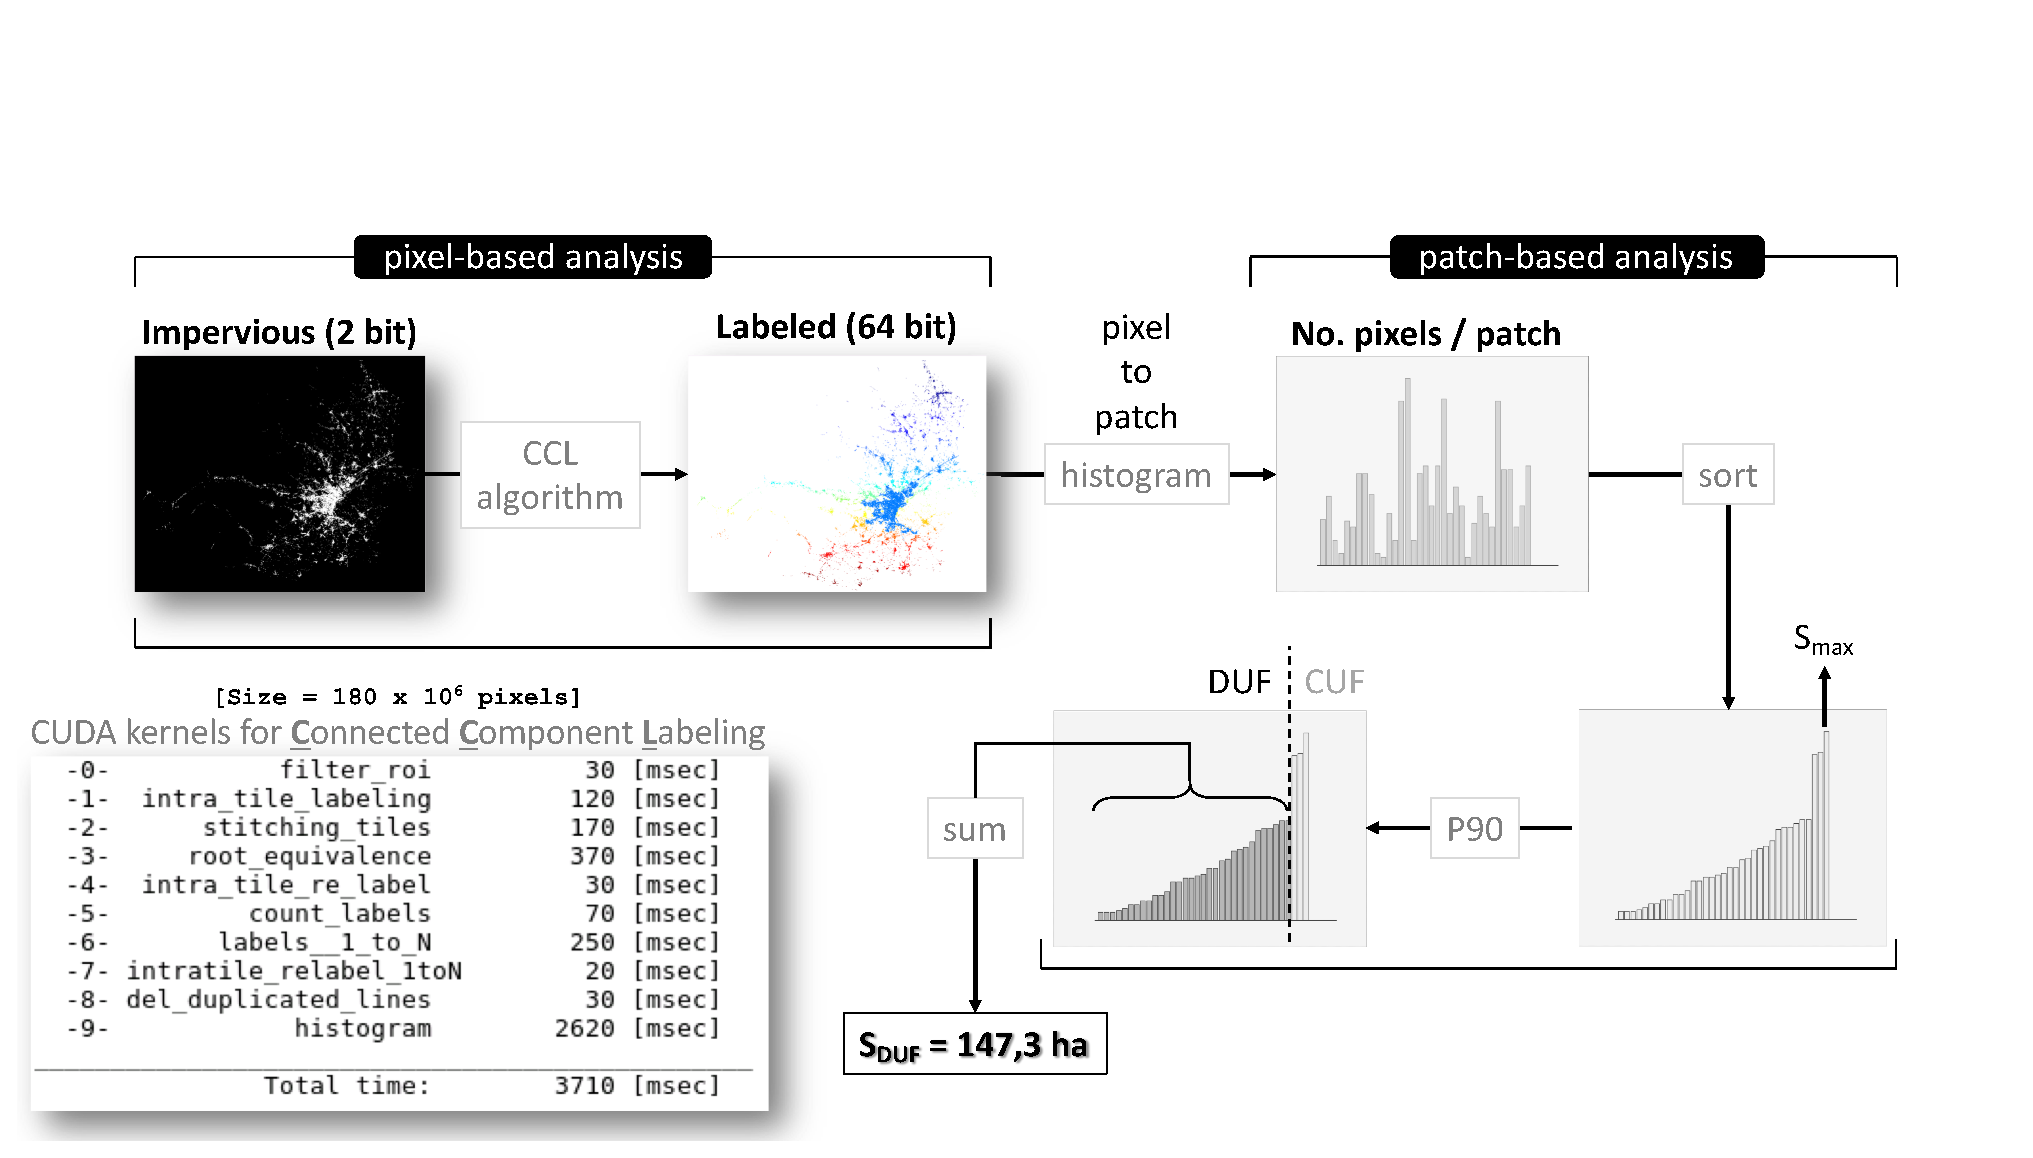
\includegraphics[width=500pt]{03_DUF_explanation.eps}}
    \caption{ \DIFaddFL{The calculation of the discontinuous urban fabric surface ($S_{DUF}$) developed within Soil Monitor cyber-infrastructure. 
    The pixel-based calculations are perfomed on the GPU card running a connected component labelling algorithm written in CUDA-C. 
    The patch-based calculations are performed on the CPU by Java code.
    The elapsed times in the box of CUDA kernels refer to an image of size $180 \times 10^6$ pixels using a NVIDIA TESLA C2075 GPU card.
    ( DUF = discontinuous urban fabric; CUF = continuous urban fabric; $S_{max}$ = largest urban patch surface)}} \label{fig:ccl}
\end{figure}
\subsection{\DIFadd{Quantitative monitoring and analysis on three Italian case studies using Soil Monitor}}\label{sec:caseStudies}

\subsubsection{ \DIFadd{Land use/cover monitoring for whole Italy }} \label{sec:caseIT}
\DIFadd{Land use/cover pattern is the consequence of natural and socio-economic factors and their utilization by man in time and space.
Knowledge about land use/cover, for instance assisted by monitoring, and potentialities for optimal use are crucial for the selection, planning and implementation of land use schemes that meet both the increasing demands for basic human needs and %DIF > welfare.
the changing demands of increasing population.
Consequently, accurate monitoring of the temporal changes of the land surface state is important to understand the relationship between man and nature and to provide decision makers with relevant information.
The information on vegetation change is probably the most important of these relationships and will be used in the following analysis.
The type and evolution of vegetation cover can be a powerful indicator of the magnitude of land degradation that is assessed by comparing land use/cover maps over different times.
Although land cover reflects the physical characteristics of earth's surface and differently land use refers to the way in which land has been used by humans, it is not possible to keep them separated in the following analysis.
}

\DIFadd{In }\DIFaddend Italy, the monitoring of land take is \DIFdelbegin \DIFdel{ensured }\DIFdelend \DIFaddbegin \DIFadd{accounted for }\DIFaddend by the National System for the Protection of the Environment (SNPA) as established by \DIFdelbegin \DIFdel{L.132}\DIFdelend \DIFaddbegin \DIFadd{the entry into force of law 132}\DIFaddend /2016.
Accordingly, the SNPA is coordinated by ISPRA and involves all Italian Environmental Protection Agencies \DIFdelbegin \DIFdel{(ARPA-APPA)}\DIFdelend \DIFaddbegin \DIFadd{working at the regional level}\DIFaddend . 
This monitoring is scheduled in order to have an annually updated picture of the soil sealing evolution (e.g. ISPRA 2016, 2018) and the dynamics of land transformation and urban development, which is done through the production of thematic maps and the development of specific indicators. 
\DIFdelbegin \DIFdel{The L.132}\DIFdelend \DIFaddbegin \DIFadd{Law 132}\DIFaddend /2016 states that the SNPA must ensure such monitoring through monitoring points/networks or earth observation techniques (e.g. Copernicus).
In performing such monitoring, ISPRA and SNPA face two major problems: (i) difficult interaction with over 8000 Italian municipalities and (ii) the lack of awareness \DIFdelbegin \DIFdel{about the crucial importance of the soil sealing land degradation process by citizens and other public authorities}\DIFdelend \DIFaddbegin \DIFadd{by citizens and other public authorities about the impact of soil sealing on land degradation}\DIFaddend .

In this framework, Soil Monitor can indeed represent an important step forward in land \DIFdelbegin \DIFdel{take and land usemonitoring.
Moreover, any administrative unit can monitor land take and land use}\DIFdelend \DIFaddbegin \DIFadd{use}\DIFaddend /cover \DIFdelbegin \DIFdel{evolution through maps (e.g. showing the new urbanized area), numeric or graphical representation of some indicators, and comparing indicators between different years, for instance, to evaluate changes in urban development or in the fragmentation of the rural territory.
}%DIFDELCMD < 

%DIFDELCMD < %%%
\DIFdel{Furthermore, it is important to highlight that Soil Monitor contributes to the analysisof soil sealing through standardized approaches, thus avoiding the current trend of creating several customised indexes produced by many users as it currently happens in using the large flexibility offered by many kinds of desktop software (e.
g. fragstat}\footnote{\DIFdel{https://www.umass.edu/landeco/research/fragstats/fragstats.html}}%DIFAUXCMD
\addtocounter{footnote}{-1}%DIFAUXCMD
\DIFdel{). 
}%DIFDELCMD < 

%DIFDELCMD < %%%
\DIFdel{A case of use of the platform is given }\DIFdelend \DIFaddbegin \DIFadd{quantitative monitoring and analysis.
To show the results }\DIFaddend in Figure \ref{fig:caseIT}, \DIFdelbegin \DIFdel{where the }\DIFdelend \DIFaddbegin \DIFadd{the calculation of the }\DIFaddend matrix of land use\DIFdelbegin \DIFdel{and land cover changes (LULC) for all of Italy has been analysed and reported. 
}%DIFDELCMD < 

%%DIFDELCMD < 
%\begin{figure}
%[t]
%%DIFDELCMD <     %%%
%%DIF <  \includegraphics[width,,height=15pc,draft]
%    %DIFDELCMD < \centerline{\includegraphics[width=450pt]{Figure04.pdf}}
%%DIFDELCMD <     %%%
%%DIFDELCMD < \caption{%
%{%DIFAUXCMD
%\DIFdelFL{The interactive change matrix for Italy between 1954 and 2012.
%    The changes in both the chart and the map are depicted by colours, each of which is associated with the class in the reference year (1954) consumed by artificial surfaces in the current year (2012) }} %DIFAUXCMD
%%DIFDELCMD < %DIFDELCMD < \label{fig:caseIT}%%%
%%DIFDELCMD < 
%\end{figure}
%%DIFDELCMD < 

%DIFDELCMD < %%%
\DIFdel{Additionally, any RoI can be freely selected by the user and any portion (administrative levels included) of the Italian territory can be analysed. Consequently, the change matrix calculation is highly demanding due to the high number of classes that can be included (in particular, using CLC at Level 3), to the large spatial extent and }\DIFdelend \DIFaddbegin \DIFadd{/cover change was submitted to the platform using }\DIFaddend the \DIFdelbegin \DIFdel{high spatial detail; therefore, a multi-GPU approach was developed, through CUDA streams, to further accelerate demanding requests thus enabling real-time queries}\DIFdelend \DIFaddbegin \DIFadd{whole Italy as RoI,
Touring and CLC as basic data and
the two contrasting yeas 1954 and 2012 as time filters}\DIFaddend .
The system \DIFdelbegin \DIFdel{produces a table with all }\DIFdelend \DIFaddbegin \DIFadd{produced an interactive change matrix with the }\DIFaddend land use changes \DIFdelbegin \DIFdel{for two contrasting years. 
For instance, in Fig 4a, all the changes of state contributing to }\DIFdelend \DIFaddbegin \DIFadd{between 13 different classes for }\DIFaddend the \DIFdelbegin \textit{\DIFdel{artificial surfaces}} %DIFAUXCMD
\DIFdel{class between two different years was selected. 
In our case, the largest }\DIFdelend \DIFaddbegin \DIFadd{entire country.
From these data (see Figure \ref{fig:caseIT}}\textit{\DIFadd{a}} \DIFadd{and }\textit{\DIFadd{b}}\DIFadd{) it is very interesting to emphasise that the }\DIFaddend land use class \DIFaddbegin \DIFadd{mostly }\DIFaddend affected by new \DIFdelbegin \DIFdel{artificial surfaces }\DIFdelend \DIFaddbegin \textit{\DIFadd{artificial surfaces}} \DIFaddend is the \textit{complex cultivation patterns} \DIFdelbegin \DIFdel{class, }\DIFdelend with a loss of \DIFdelbegin \DIFdel{about }\DIFdelend 418\DIFdelbegin \DIFdel{thousand hectares from 1954 to 2012. 
Accordingly,the key innovation in Soil Monitor consists of an interactive }\DIFdelend \DIFaddbegin \DIFadd{,604 ha, that is the 26.72\% of transformation into }\textit{\DIFadd{artificial surfaces}} \DIFadd{in whole Italy from 50's to 2012 was possible due to the consumption of }\textit{\DIFadd{complex cultivation patterns}}\DIFadd{.
Since the }\DIFaddend matrix of changes \DIFdelbegin \DIFdel{, which can be dynamically queried fixing a column (i.e. class of }\textit{\DIFdel{artificial surfaces}} %DIFAUXCMD
\DIFdel{in 2012) or a row (i.e. a class of any other land use in 1954) , getting a chart and a map of changes on demand. 
Moreover, a pie diagram provides an immediate }\DIFdelend \DIFaddbegin \DIFadd{generated by Soil Monitor is interactive, the click on the column of artificial surfaces produced either a pie chart (not shown) enabling an immediate and intuitive }\DIFaddend quantification of the changes by classes contributing to \textit{artificial surfaces} \DIFdelbegin \DIFdel{(Figure \ref{fig:caseIT}b).
The map depicts the geography of changes providing details till the pixel level; it }\DIFdelend \DIFaddbegin \DIFadd{or an image map where it is possible to see where these changes have occurred (see the zoom of such a map in Figure \ref{fig:caseIT}}\textit{\DIFadd{c}}\DIFadd{).
It }\DIFaddend is possible to observe that the largest changes from \DIFdelbegin \DIFdel{complex cultivation patterns to artificial areas occurring }\DIFdelend \DIFaddbegin \textit{\DIFadd{complex cultivation patterns}} \DIFadd{to }\textit{\DIFadd{artificial surfaces}} \DIFadd{occurred }\DIFaddend at the fringes of earlier urban centres\DIFdelbegin \DIFdel{(Figure \ref{fig:caseIT}c) . 
This geospatial analysis, especially when used to compare and analyse LULC changes between more recent years, is a very powerful tool.
It provides very detailed geospatial information about the }\DIFdelend \DIFaddbegin \DIFadd{.
}


\begin{figure}
[t] %DIF >  FIGURE 04
    \centerline{\includegraphics[width=450pt]{04_caso_nazionale.eps}}
    \caption{ \DIFaddFL{The interactive change matrix calculation for whole Italy between 1954 and 2012.
    (a) The matrix of changes in hectares (ha) with particular focus on the column of }\textit{\DIFaddFL{artificial surfaces}} \DIFaddFL{(year 2012) with contributions coming from other classes (year 1954).
    (b) Same matrix of change as in (a) but expressed in percentage of the overall Italian area (except in parenthesis where percentages refer to the total of the class in header).
    (c) Map of }\textit{\DIFaddFL{artificial surfaces}} \DIFaddFL{(year 2012) with contributions coming from other classes (year 1954).
    }} \label{fig:caseIT}
\end{figure}
\textit{\DIFadd{Forests}} \DIFadd{covers one third (33.66\%) of the Italian area on 2012 and is one of the most conservative classes with respect to land take, since it only contributed by 4.41\% to the overall transformation into }\textit{\DIFadd{artificial surfaces}} \DIFadd{(the 0.23\% of total area).
Considering the above evidences along with the analysis of other }\DIFaddend land use classes, \DIFdelbegin \DIFdel{which have been affected more by urbanization, and it possibly highlights those LULC classes that have a major risk to be affected by new urbanization in the near future.
Further, the new urbanization depicted in Fig. 4c shows that the land use mostly affected by urbanization is the less specialised one, namely }\DIFdelend \DIFaddbegin \DIFadd{as a concluding remark the classes characterised by a lower level of specialization are the most fragile with respect to new land take.
}\textit{\DIFadd{Complex cultivation patters}} \DIFadd{and }\textit{\DIFadd{non-irrigated arable land}} \DIFadd{have suffered a tremendous general trade off with different other classes, because only about a quarter and half of their surfaces, respectively, remained unchanged between 1954 and 2012.
It quantifies the great impact of man pressure in solely 60 years, considering that }\textit{\DIFadd{complex cultivation patters}} \DIFadd{and }\textit{\DIFadd{non-irrigated arable land}} \DIFadd{together cover about the 42\% of the Italian territory.
On the contrary instead, classes such as }\DIFaddend \textit{\DIFdelbegin \DIFdel{complex cultivation patterns}\DIFdelend \DIFaddbegin \DIFadd{vineyards}\DIFaddend }\DIFaddbegin \DIFadd{, }\textit{\DIFadd{olive groves}} \DIFadd{and }\textit{\DIFadd{fruit trees and berry plantations}} \DIFadd{are better defending, in particular against the land take aggression}\DIFaddend .
Therefore, higher specialization in agriculture would perhaps produce more resilient \DIFdelbegin \DIFdel{LULC }\DIFdelend \DIFaddbegin \DIFadd{land use/cover }\DIFaddend classes to challenge new land take pressures.

\DIFdelbegin \subsection{\DIFdel{The case study of territorial plan (PTCP)}}
%DIFAUXCMD
\addtocounter{subsection}{-1}%DIFAUXCMD
\DIFdelend \DIFaddbegin \DIFadd{By means of the Soil Monitor platform, we analysed the changes between 1954 and 2012 in further detail
for each separate Italian administrative region, with particular emphasis on quantifying changes in }\textit{\DIFadd{artificial surfaces}}\DIFadd{, }\textit{\DIFadd{forests}} \DIFadd{and }\textit{\DIFadd{complex cultivation patterns}} \DIFadd{(see Figure \ref{fig:caseIT_graphs}a).
Those regions, such as Lombardia and Veneto, experiencing a large land take (about 10\% and 8\% of their regional areas, respectively) are also most affected by a loss in }\textit{\DIFadd{complex cultivation patterns}}\DIFadd{.
On the contrary, regions affected by weak land take dynamics, such as Molise, Valle D'Aosta and Liguria show a better preservation of the }\textit{\DIFadd{complex cultivation patterns}} \DIFadd{class.
}
\begin{figure}
    \centerline{ \includegraphics[width=450pt]{05_caso_nazionale_grafici.eps} }
    \caption{\DIFaddFL{Breakdown of changes between 1954 and 2012 by region assuming the regional area as total within each region.
             (a) Impact of regional changes on }\textit{\DIFaddFL{artificial surfaces}}\DIFaddFL{, }\textit{\DIFaddFL{forests}} \DIFaddFL{and }\textit{\DIFaddFL{complex cultivation patterns}}\DIFaddFL{.
             (b) Regional changes in the trade off between }\textit{\DIFaddFL{forests}} \DIFaddFL{and }\textit{\DIFaddFL{complex cultivation patterns}} \DIFaddFL{with }\textit{\DIFaddFL{artificial surfaces}}\DIFaddFL{.}}
    \label{fig:caseIT_graphs}
\end{figure}
\DIFadd{A close-up of the above evidences is reported in Figure \ref{fig:caseIT_graphs}(b) where we quantified the impact of artificial surfaces over }\textit{\DIFadd{forest}} \DIFadd{and }\textit{\DIFadd{complex cultivation patterns}}\DIFadd{. 
The areas covered by }\textit{\DIFadd{complex cultivation patterns}} \DIFadd{have been strongly challenged by land take in regions such as Veneto, Lombardia, Emilia Romagna and Friuli Venezia Giulia which have also the largest gross domestic production in Italy.
}


\subsubsection{\DIFadd{The territorial plan at the province level (PTCP)}}
\label{sec:casePROV}
\DIFaddend In Italy, the reference administrative level for urban planning coordination in terms of environmental issues is the province law 142/1990. 
Thus, it is the key geographical level to challenge land take. 
However, this situation somehow remained unchanged after law 56/2014 (rules on metropolitan cities) and even after the constitutional referendum that transfers the competences of the provinces to the regions (4 December 2016).
Currently, provinces (albeit in specific cases, metropolitan cities and regions) carry out the fundamental coordinating role for territorial planning, protection, and enhancement. 
Moreover, typically, this is performed through the ''territorial plan of coordination at province level'' called PTCP (Piano Territoriale di Coordinamento Provinciale), which aims at: (i) land use regulation to protect natural areas and cultural heritage; (ii) guidance and implementation of subordinate planning producing general guidelines to be followed by municipalities in their local plans; (iii) coordination of planning activities by local authorities in order to achieve a rational organization of the provincial spaces.

In the last decades, there have been many regional laws and provincial policies in Italy, highlighting the need to mitigate land take, thus guaranteeing the preservation of the landscape and its ecosystem services. 
In such a framework, the crucial need to support the PTCP planning in order to truly mitigate soil sealing is evident. 
This government level is \DIFdelbegin \DIFdel{farther to the pressures  }\DIFdelend \DIFaddbegin \DIFadd{not under the major pressure }\DIFaddend of pro-growth policies, which are instead strongly grounded in the city and town leading coalitions.
Therefore, Soil Monitor can help implement these regulative ambitions.
For each Italian province, the platform allows carrying out a detailed analysis of both recent and past urbanization with the production of \DIFdelbegin \DIFdel{indices }\DIFdelend \DIFaddbegin \DIFadd{metrics }\DIFaddend and maps identifying the main soil sealing criticalities within the territory.
Moreover, Soil Monitor classifies administrative units on the base of urban sprawl, giving the opportunity to the governing body to define targeted and selected geographies of the densification policy.

\DIFdelbegin \DIFdel{A case of use of the platform at the provincial level is reported in Figure \ref{fig:casePROV}, which shows a plot of three indicators, namely LCDI, RMPS, and ED (presented in Table \ref{tab:IMPclasses}), describing the model of urban development of the five provincial capitals in Campania Region: Avellino, Benevento, Caserta, Napoli, and Salerno (Figure \ref{fig:casePROV}a). 
The combination of the results of the three indicators helps in evaluating the degree of urban dispersion and, for instance, enables differentiating monocentric from polycentric municipalities. 
As such, Caserta, Napoli, and Salerno --- having a LCPI larger than 70\% --- are monocentric and compacted, while Avellino and Benevento have a clearly polycentric distribution.
}%DIFDELCMD < 

%%DIFDELCMD < 
%\begin{figure}
%[t]
%%DIFDELCMD <     %%%
%%DIF <  \includegraphics[width,,height=15pc,draft]
%    %DIFDELCMD < \centerline{\includegraphics[width=250pt]{Figure05.pdf}}
%%DIFDELCMD <     %%%
%%DIFDELCMD < \caption{%
%{%DIFAUXCMD
%\DIFdelFL{Soil Monitor supports the analysis at the level of the territorial plan of coordination (PTCP). }} %DIFAUXCMD
%%DIFDELCMD < %DIFDELCMD < \label{fig:casePROV}%%%
%%DIFDELCMD < 
%\end{figure}
%%DIFDELCMD < 

%DIFDELCMD < %%%
\DIFdelend In Figure \ref{fig:casePROV} \DIFdelbegin \DIFdel{b }\DIFdelend a quantitative map of the rural fragmentation is given for the Milano province, an area very dynamic with a high per capita income and high residential and infrastructure pressure. 
This map is very important because it enables the quantification of each point in the landscape to the degree of its rural integrity. 
Accordingly, calculations are performed on-the-fly, enabling \DIFdelbegin \DIFdel{the }\DIFdelend planners to freely decide the radius of their analysis\DIFdelbegin \DIFdel{(size of kernel to be processed)}\DIFdelend .
Generally, a smaller radius (e.g. 100 m) is useful for detailed urban planning at the scale of a specific intervention, such as a new green corridor or a new development.
By contrast, a fragmentation analysis performed with a large radius (e.g. >500 m) produces an output affected by very large areas, either urban or natural. 
Thus, this analysis is useful to describe major geographical trends of rural integrity.
\DIFdelbegin %DIFDELCMD < 

%DIFDELCMD < %%%
\DIFdelend The output from the above analysis can be profitably used to better plan future urban development, thus avoiding new fragmentation of rural areas, especially those with high integrity, and to plan where to place new green infrastructures connecting rural areas with high rural integrity.

\DIFdelbegin \subsection{\DIFdel{The case study of the municipal plan (PUC)}}
%DIFAUXCMD
\addtocounter{subsection}{-1}%DIFAUXCMD
\DIFdelend \DIFaddbegin 
\begin{figure}
[t] %DIF >  FIGURE 05
    \centerline{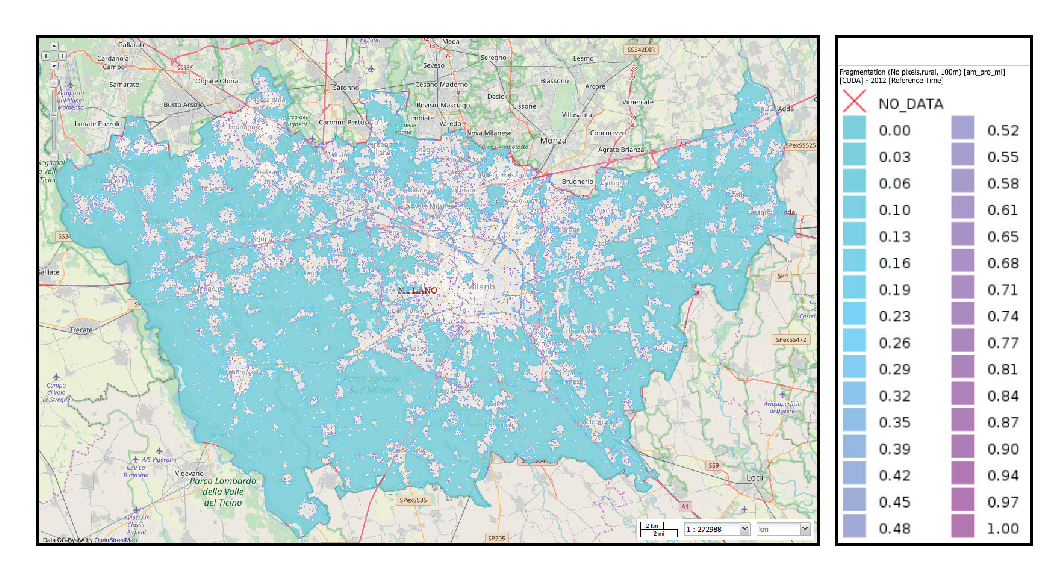
\includegraphics[width=450pt]{06_caso_provinciale.eps}}
    \caption{ \DIFaddFL{Map of rural fragmentation calculated in the province of Milan on 2012. }} \label{fig:casePROV}
\end{figure}

\subsubsection{ \DIFadd{Planning at the municipal level (PUC) }}
\label{sec:caseCOM}

\DIFaddend The municipal urbanization plan (PUC) is a tool for the management of the Italian municipal territory, which consists of cartographic and technical documents along with regulations for the management of urban and territorial transformations within the municipality.
\DIFdelbegin %DIFDELCMD < 

%DIFDELCMD < %%%
\DIFdelend The PUC stems from the old well known \DIFdelbegin \DIFdel{general regulatory plan }\DIFdelend \DIFaddbegin \DIFadd{General Regulatory Plan }\DIFaddend (PRG established by Italian law 1150/1942); it is produced by urban planners assisted by experts from other fields (e.g. environmental scientists, pedologists, geologists, and lawyers).
\DIFdelbegin %DIFDELCMD < 

%DIFDELCMD < %%%
\DIFdel{Therefore, the PUC must have }\DIFdelend \DIFaddbegin \DIFadd{Although the PUC has no duration limitations, it is periodically reviewed and has }\DIFaddend a long series of requirements\DIFaddbegin \DIFadd{, such as}\DIFaddend : (i) the identification and discipline of land uses; (ii) the subdivision of the territory into zones with different and complementary uses; (iii) the protection and enhancement of natural, landscape, and historical-cultural heritage. 
\DIFdelbegin \DIFdel{Although the PUC has no duration limitations, it is periodically reviewed.
}\DIFdelend Moreover, since the PUC is the planning document closer to operational urban activities, it is important for Soil Monitor to be used at \DIFdelbegin \DIFdel{this scale. 
At }\DIFdelend the municipal scale, \DIFdelbegin \DIFdel{Soil Monitor enables performing a scenario analysis by simulating different urban interventions of green corridors by evaluating the effects of such interventions on the rural integrity; the system also allows the visualization and connect planning information with other environmental maps such as landscape constraints.
}\DIFdelend \DIFaddbegin \DIFadd{where it enables (i) to analyse of a set of indicators of urban sprawl and of urban development, (ii) to support municipalities in having geospatial information useful for fulfilling the PUC requirements.
}\DIFaddend 

%\DIFdelbegin %DIFDELCMD < 
%\begin{figure}
%[t]
%%DIFDELCMD <     %%%
%%DIF <  \includegraphics[width,,height=15pc,draft]
%    %DIFDELCMD < \centerline{\includegraphics[width=450pt]{Figure06.pdf}}
%%DIFDELCMD <     %%%
%\DIFdelendFL \DIFaddbeginFL \DIFaddFL{In the following it is shown the value of Soil Monitor in two different domains: (i) in quantification and analysis of land take dynamics and (ii) in municipality planning support. 
%}

\DIFaddFL{The study of quantification and analysis of land take dynamics at municipality level is presented in Figure \ref{fig:caseCOM_urbDev}, where a set of indicators for all the municipalities of the province of Napoli are reported for the quantitative analysis.
The statistics on }\textit{\DIFaddFL{Largest Class Patch Index}} \DIFaddFL{(LCPI) , }\textit{\DIFaddFL{Residual Mean Patch Surface}} \DIFaddFL{(RMPS) and }\textit{\DIFaddFL{Edge Density}} \DIFaddFL{(ED) metrics highlight a very large variation between the municipalities (Figure \ref{fig:caseCOM_urbDev}a).
More specifically, Casavatore shows a strong monocentric urban development with the highest LCPI value (LCPI: 99.98), while Monte di Procida has the most pronounced
polycentric nature with many small urban nuclei (RMPS: 1.18).
An analysis on edge density --- which is a good proxy of urban dispersion (e.g. \mbox{%DIFAUXCMD
\citealp{SCHWARZ2010}}%DIFAUXCMD
) --- shows that the rural mountain settlement of Agerola has the highest urban dispersion (ED: 1174) while the almost fully urbanized area of Casavatore shows the lowest urban dispersion trend (ED: 74).
Therefore, it is evident that these data requires further integration with other indexes such as the fraction of urbanized area and the population.
In Figure \ref{fig:caseCOM_urbDev}b we report a diagram quantifying ED for the municipalities of Napoli's province.
There are over 22 municipalities with a very high (>600) edge density and many of them refer to summer-based touristic sites in hilly and mountain sites (Agerola, Serra Fontana, Annacapri, Massalubrense, Vico Equense, Barano d'Ischia, Capri, Forio, Piano di Sorrento, etc.).
While the municipalities with the lower edge density (Casavatore, Arzano, Cardito, Melito di Napoli Portici) are not rural sites but rather strongly urbanized cities with very minimal and concentrated rural areas (thus low ED metric).
}
\begin{figure}
    \centerline{
        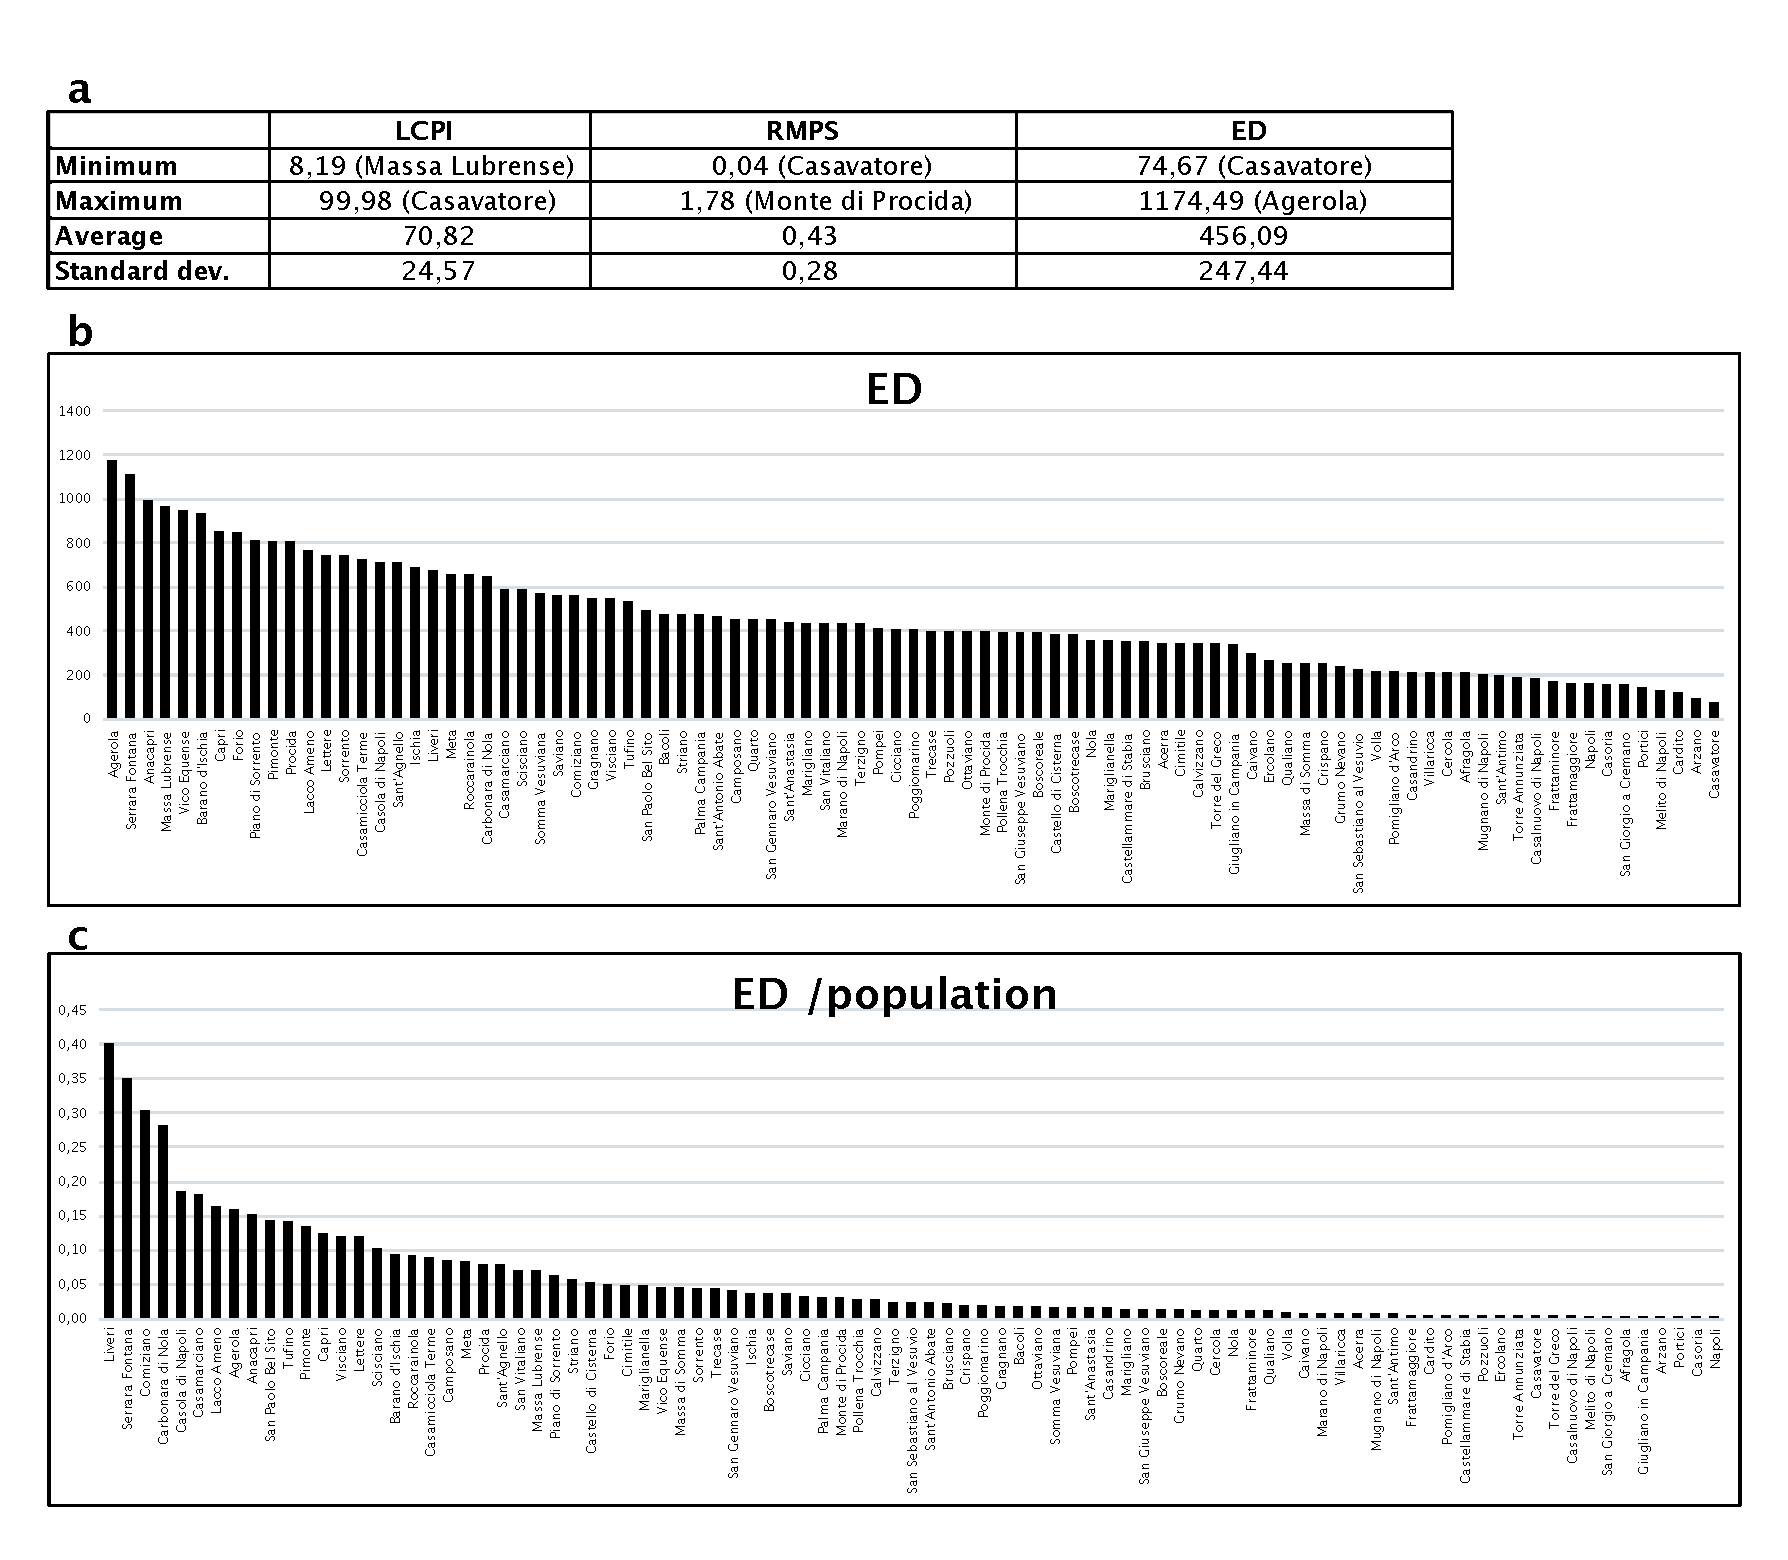
\includegraphics[width=450pt]{08_caso_comunale_tabella_grafici.eps}
    }
    \DIFaddendFL \caption{\DIFdelbeginFL \DIFdelFL{Soil Monitor supports the }\DIFdelendFL \DIFaddbeginFL \DIFaddFL{Quantitative }\DIFaddendFL analysis \DIFdelbeginFL \DIFdelFL{at }\DIFdelendFL \DIFaddbeginFL \DIFaddFL{of }\DIFaddendFL the \DIFdelbeginFL \DIFdelFL{level }\DIFdelendFL \DIFaddbeginFL \DIFaddFL{urban development }\DIFaddendFL of \DIFaddbeginFL \DIFaddFL{all municipalities within }\DIFaddendFL the \DIFdelbeginFL \DIFdelFL{municipal urbanization plan }\DIFdelendFL \DIFaddbeginFL \DIFaddFL{province on Napoli }\DIFaddendFL (\DIFdelbeginFL \DIFdelFL{PUC}\DIFdelendFL \DIFaddbeginFL \DIFaddFL{year 2012}\DIFaddendFL ).
             \DIFaddbeginFL \DIFaddFL{(a) Summary statistics of metrics LCPI, RMPS and ED.
             (b) Edge density bar plot.
             (c) Bar plot of the ratio between edge density and population size.
             (LCPI: Largest Class Patch Index; 
             RMPS: Residual Mean Patch Surface; 
             ED: Edge Density)
            }\DIFaddendFL }
    \DIFdelbeginFL %DIFDELCMD < %DIFDELCMD < \label{fig:caseCOM}%%%
%DIFDELCMD < %%%
\DIFdelendFL \DIFaddbeginFL \label{fig:caseCOM_urbDev}
\DIFaddendFL 
\end{figure}

A \DIFdelbegin \DIFdel{case of use of the platform at the municipality level is reported in Figure \ref{fig:caseCOM}}\DIFdelend \DIFaddbegin \DIFadd{more detailed analysis was then performed on the ratio between edge density and population size to highlight municipalities having a strong urban dispersion despite low population (Figure \ref{fig:caseCOM_urbDev}c).
This analysis points out that many small municipalities (e.g. Liveri, Comiziano, Carbonara di Nola,Casola di Napoli) --- well immerse in the rural environment and not having a touristic value --- show unexpected high ED/population values thus depicting a strong aggression of rural areas despite the very low population pressure.
From all analysis above it is evident the high explication value of the above indexes to better understand the urban development and, even more importantly, the impact of land take at municipality level.
}

\DIFadd{In addition to the analysis of the land take dynamics given above, an analysis to support urban planning at the municipality level using Soil Monitor is provided in the following (Figure \ref{fig:caseCOM_Ercolano})}\DIFaddend .
The city of Ercolano is located between the Vesuvius volcano and the \DIFdelbegin \DIFdel{sea}\DIFdelend \DIFaddbegin \DIFadd{Tyrrhenian Sea}\DIFaddend , has a high population density, and is devoted to tourism owing to historical sites and spot of high-quality agriculture (e.g. wine, fruit trees, and flowers). 
Therefore, the user can get a quantification of the evolutive trajectories that led to specific land use and land cover states. 
In the example shown in Figure \DIFdelbegin \DIFdel{\ref{fig:caseCOM}}\DIFdelend \DIFaddbegin \DIFadd{\ref{fig:caseCOM_Ercolano}}\DIFaddend (a, b), the amount and the geolocation of the consumption exerted by artificial surfaces is clear, above all, regarding vineyards, fruit trees, and olive orchards. 
This interpretation about the LULC evolution is accompanied by the recognition that part of the land take was very close (if not inside) to the protected areas (Figure \DIFdelbegin \DIFdel{\ref{fig:caseCOM}c}\DIFdelend \DIFaddbegin \DIFadd{\ref{fig:caseCOM_Ercolano}d}\DIFaddend ) of the Vesuvius's slopes, thereby confirming the very high pressure of urbanization not well managed by local authorities. 
Accordingly, the model of urban development was computed in the same municipality of Ercolano against other most populated cities in the Napoli province. 
Figure \DIFdelbegin \DIFdel{\ref{fig:caseCOM}d }\DIFdelend \DIFaddbegin \DIFadd{\ref{fig:caseCOM_Ercolano}(c) }\DIFaddend shows the population size and density (the left side of the table) and the indicators of model of urban development (LCPI, RMPS, and ED on the right side of the table), depicting the main urban trends in the Napoli province.
\DIFdelbegin \DIFdel{The results reported in Figure \ref{fig:caseCOM} }\DIFdelend \DIFaddbegin \DIFadd{These results }\DIFaddend are limited examples of the \DIFdelbegin \DIFdel{information that can possibly }\DIFdelend \DIFaddbegin \DIFadd{awareness building that can }\DIFaddend be achieved using Soil Monitor, which \DIFdelbegin \DIFdel{can be profitably used to enhance }\DIFdelend \DIFaddbegin \DIFadd{in turn profitably supports }\DIFaddend the definition and implementation of plans at the municipality scale (PUC in Italy).
This finding becomes much more important considering Soil Monitor is operational over the entire Italian territory with more than eight thousand municipalities.

\DIFdelbegin \section{\DIFdel{Conclusions}}
%DIFAUXCMD
\addtocounter{section}{-1}%DIFAUXCMD
\DIFdel{Soil sealing mitigation implemented through best land spatial planning practices is a very virtuous goal, but it is also one of the greatest challenges of the modern world. 
In fact, high quantity of information can only be accessed through satellite and drones, etc. concerning, for example, the agricultural, forestry, environmental, and spatial planning sectors is simply not sufficient to face the complexity of this challenge. 
}%DIFDELCMD < 

%DIFDELCMD < %%%
\DIFdel{This work shows that starting from the problem statement in a specific research domain, it is feasible to combine recent achievements in terms of data, models, indicators , WebGIS, and HPC technologies to produce an integrated geospatial cyberinfrastructure available on the web, aiming to account and mitigate the continual soil sealing worldwide. 
The proposed application called SMapp, which is freely accessible via an internet browser without the need to install any application or plugin on the local computer, aims to demonstrate that this approach is feasible}\DIFdelend \DIFaddbegin 
\begin{figure}
[t] %DIF >  FIGURE 06
    \centerline{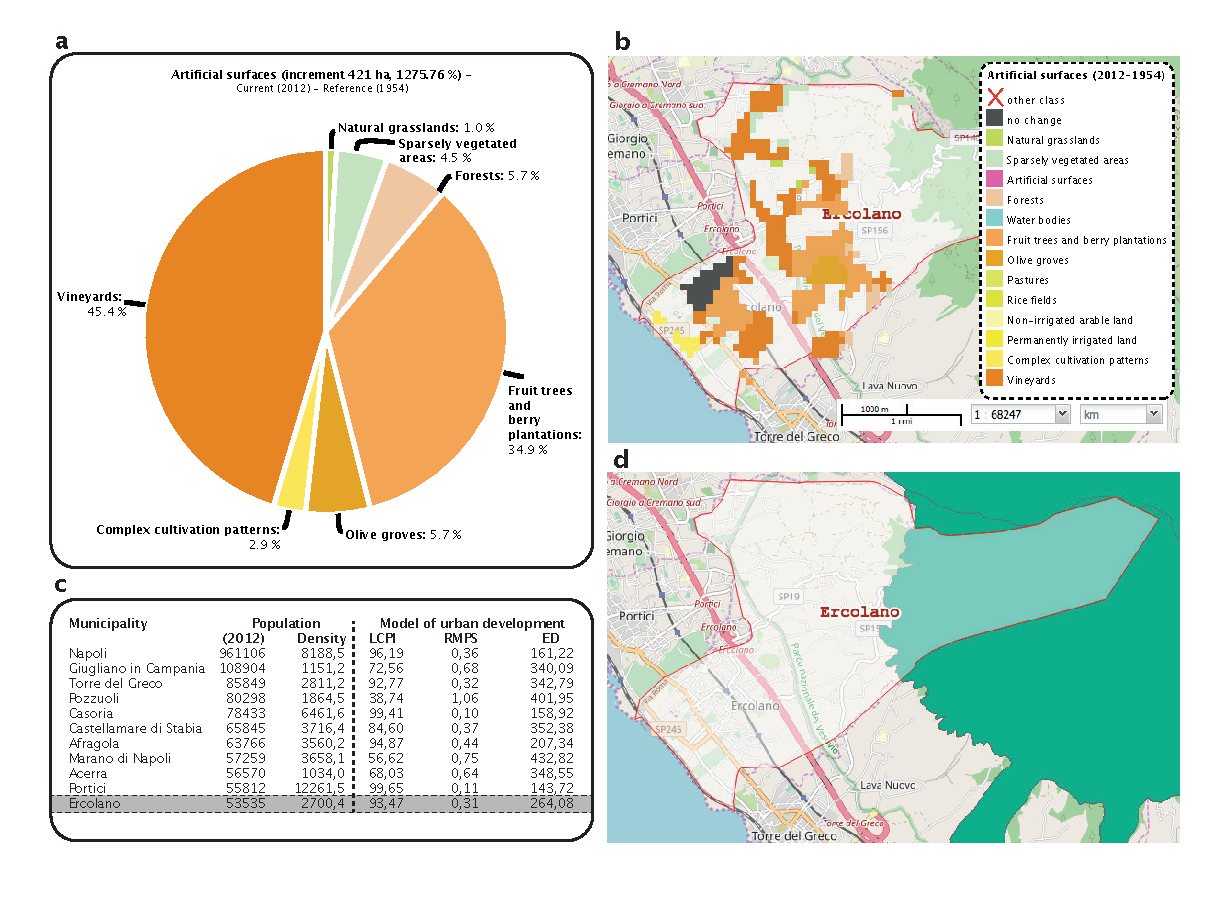
\includegraphics[width=450pt]{07_caso_comunale.eps}}
    \caption{ \DIFaddFL{Soil Monitor supports the analysis at the level of the municipal urbanization plan (PUC) in Ercolano municipality.
              (a) Pie chart of the LULC changes in Ercolano towards artificial surfaces in 2012 from all other classes in 1954.
              (b) Image map of the changes in Ercolano depicted in (a).
              (c) Data and metrics supporting the quantitative analysis at the municipality level.
              (d) The Ercolano RoI in contrast with the landscape constraints given by Vesusius national park (dark green). }}
    \label{fig:caseCOM_Ercolano}
\end{figure}
\subsection{\DIFadd{Final discussion}}
\DIFadd{Soil Monitor is designed to address the accountancy of soil sealing through different indicators providing operational support to urban planners, decision makers and multi stakeholders involved in landscape planning and interested in evaluating the impact of soil sealing. 
This specific contribution required a different approach, the result of which is the Soil Monitor geospatial cyber-infrastructure. 
A set of indicators can be calculated in real-time using either Italian administrative levels (NUTS2, NUTS3, and LAU2) or user-drawn Regions of Interest (RoI)}\DIFaddend . 
Moreover, \DIFdelbegin \DIFdel{it takes advantage of the combination of updated high spatial resolution data on imperviousness available in Italyowing to ISPRA with tailored codes written in CUDA to gain embarrassingly parallel applications, thereby enabling a highly detailed }\DIFdelend \DIFaddbegin \DIFadd{Soil Monitor uses high resolution layers produced every year by ISPRA (Italian Institute for Environmental Protection and Research) since 2015 for drawing up their yearly soil sealing report in Italy. 
Thus, owing to the high-performance computing embedded in its cyber-infrastructure, Soil Monitor enables real-time geospatial processing while preserving a high spatial detail of the }\DIFaddend analysis over large \DIFdelbegin \DIFdel{geographical extents.
Additionally, the combination of WebGIS with GPU computing running on-the-fly geospatial processing puts Soil Monitorat the fringe of research and development. 
Further, the GPU parallelism model enables a higher speedup than the CPU counterpart, at both a lower cost and a lower power consumption, with the main limitation being the requirement to design and write new codes from scratch.
}\DIFdelend \DIFaddbegin \DIFadd{areas (till LAU2, but it can scale according to available hardware).
This combination of features has an intrinsic vast potential for being used in operational spatial planning as testified by the results presented in this work. 
}\DIFaddend 

\DIFdelbegin \DIFdel{Nevertheless, the proposed platform still remains a prototype from research that can be used for any area of }\DIFdelend \DIFaddbegin \DIFadd{Despite the huge endeavour spent on the logic tier to have GPU computing on board of Soil Monitor, }\DIFaddend the \DIFdelbegin \DIFdel{Italian territory. 
Subsequently, it can be seen as a democratic tool for creating reports that can catch the evolution of land use trajectories and connected land degradation interpretations about the ongoing land degradation processes.
}%DIFDELCMD < 

%DIFDELCMD < %%%
\DIFdel{Despite the above positive statements, it is also essential to underline that the construction, maintenance, and updating of the infrastructure requires the following:
}%DIFDELCMD < \begin{enumerate}[label=(\roman*)]
%DIFDELCMD <     \item %%%
\DIFdel{Above all, a more comprehensive and detailed data on soils which, at least in Italy, are still missing to account for land degradation surface quantity.
This information is critical to discriminate }\DIFdelend \DIFaddbegin \DIFadd{platform shows some important limitations caused by constraints in the data.
First, one main limitation is the lack of soil information underpinning the analysis, %DIF >  in Soil Monitor, 
such as the lack of different qualities of soils and their spatial distribution in the scenario analysis.
But unfortunately there not exists a detailed and homogeneous soil map for whole Italy.
To smoothly mitigate the fundamental shortcoming of not having soil information and to help discriminating }\DIFaddend between the different land qualities vulnerable to land take\DIFdelbegin \DIFdel{. 
    As such, we put soil grids by ISRIC via WMS to smoothly mitigate this fundamental shortcoming, considering }\DIFdelend \DIFaddbegin \DIFadd{, Soil Monitor shows (via WMS protocol) soil grids at 250m spatial resolution produced by ISRIC.
Attention should be drawn to }\DIFaddend the low accuracy of this \DIFdelbegin \DIFdel{grid }\DIFdelend \DIFaddbegin \DIFadd{grids }\DIFaddend with respect to the scale and \DIFaddbegin \DIFadd{the }\DIFaddend detail of the land take \DIFdelbegin \DIFdel{accountancy.
    }%DIFDELCMD < \item %%%
\DIFdel{A strong scientific effort to find the most suitable and reliable approaches for each application considering the available data.
    }%DIFDELCMD < \item %%%
\DIFdel{A strong effort to integrate different types of knowledge and technology to develop and implement web applications, according to the use of open-source components such as GeoServer and MapStore.
    }%DIFDELCMD < \item %%%
\DIFdel{Strong technical work to make the tools fully operational, mainly because of the need to provide real time answers }\DIFdelend \DIFaddbegin \DIFadd{and soil sealing analysis available in Soil Monitor.
Second, the base data (i.e. imperviousness layers) used in the analysis can have inconsistencies that Soil Monitor highlights.
It is possible to get artefacts in results %DIF > produced by Soil Monitor 
because of possible issues in the production of the data (performed by ISPRA or Copernicus), artefacts that are not caused by Soil Monitor procedures. %DIF > that does not involve Soil Monitor.
These issues can be caused by a misclassification of features over time with impervious covers unrealistically fluctuating over time }\DIFaddend (e.g. \DIFdelbegin \textit{\DIFdel{what-if}} %DIFAUXCMD
\DIFdel{modelling and scenario analysis) .
    }%DIFDELCMD < \item %%%
\DIFdel{The need for the constant maintenance of data and applications in order to keep the platform constantly and consistently operational and not obsolete.
}%DIFDELCMD < \item %%%
\DIFdel{To reinforce the
interoperability with data shared by other official providers.
The more data and thematic layers available, }\DIFdelend \DIFaddbegin \DIFadd{up and down from 0\% to 100\%) or by not detecting sealed surfaces mostly in less urbanized or rural areas.
Even though some these artefacts leads to an evident underestimation of the land degradation process, they are sporadic.
}

\DIFadd{In the presentation of the Java/JCUDA/CUDA pipeline embedded in Soil Monitor (section \ref{sec:logicTier}) 
it was shown that the JCUDA layer performs calls to }\DIFaddend the \DIFdelbegin \DIFdel{higher strength of deductions and interpretations performed during the analysis.
}%DIFDELCMD < \item %%%
\DIFdel{A more intuitive dashboard to simplify the user interaction with the visualization layer.
Indeed, because of the money constraints during the development, Soil Monitor does not ensure an easy and intuitive navigation during the job submission step. 
Nevertheless, we recognized the importance of a future effort to enhance fruition.
}%DIFDELCMD < \end{enumerate}
%DIFDELCMD < 

%DIFDELCMD < %%%
\DIFdel{Soil Monitor , by placing emphasis on landscapes, seeks to reduce the gap between policy and implementation being able to quantify and visualize (with the change in time of ) the state of }\DIFdelend \DIFaddbegin \DIFadd{CUDA kernels compiled in PTX files to address the calculation of a soil sealing metric.
The proposed pipeline is an absolute technological novelty in the implementation of geospatial decision support systems based on WebGIS and it enables the deployment of a fast geoprocessing engine capable to support a multi-user and multi-tasking web application.
To author knowledge, the
integration of high performance computing by means of the CUDA framework within web based geospatial cyber-infrastructures is absolutely new.
This is an important result that must be emphasized here not only for the technological advancement itself, but because this technology is firstly applied to soil sealing and land degradation issues and because it changes the way in which different stakeholders (citizens, technicians, professionals, policy makers, etc.) can get informed about and measure soil sealing with agreed, validated and standard methods.
}

\section{\DIFadd{Conclusions}}
\DIFadd{Soil sealing is an important form of land degradation worldwide and its mitigation implemented through best practices in spatial land planning is a very virtuous goal.
Undoubtedly, the high quantity of information that is increasingly accessible for instance through satellites and drones to tackle agricultural, forestry, environmental and spatial planning issues is simply not sufficient to face the complexity of soil sealing mitigation.
It is necessary to raise awareness in different sectors (policy, research and public) and to fund research and trans-disciplinary studies aiming to mitigate the phenomenon.
Authors call attention to the current gap in the availability of factual tools that tackle soil sealing and enable quantitative analysis, awareness building and decision making. 
The objective of this work coped with the development of a new technological solution based on geospatial cyber-infrastructures to provide an operational tool capable to study, challenge and mitigate soil sealing at different planning and spatial scales.
We demonstrated that tools such as Soil Monitor --- which is freely accessible via an internet browser without the need to install any application or plugin on the local computer --- have significant potential to fill the current gap.
The combination of WebGIS with GPU computing which runs on-the-fly geospatial processing puts Soil Monitor at the fringe of research and development. 
This kind of technology demonstrated promising capability to quantitatively measure soil sealing and to give a contribution to mitigate the %DIF > continual 
phenomenon worldwide, considering the high transferability of }\DIFaddend the \DIFdelbegin \DIFdel{land system}\DIFdelend \DIFaddbegin \DIFadd{proposed cyber-infrastructure.
Nevertheless, the proposed platform still remains a prototype from research that anyway can be used in whole Italy. 
Subsequently, it can be seen as a democratic tool for creating reports that can catch the evolution of land use trajectories and connected land degradation interpretations about the ongoing of land degradation processes}\DIFaddend .

\section*{ORCID}
Giuliano Langella \href{https://orcid.org/0000-0001-7210-0906}{ {\orcidicon{0000-0001-7210-0906}}\hspace{1.0mm} orcid.org/0000-0001-7210-0906}

\bibliography{SMapp}
\DIFdelbegin %DIFDELCMD < 

%DIFDELCMD < %%%
%DIF < The normal commands for producing the reference list are:
%DIF < \begin{verbatim}
%DIF < \begin{thebibliography}{99}
%DIF < \bibitem{<x-ref label>}
%DIF <          <Reference details>
%DIF < \end{thebibliography}
%DIF < \end{verbatim}
\DIFdelend 

\end{document}